% Options for packages loaded elsewhere
% Options for packages loaded elsewhere
\PassOptionsToPackage{unicode}{hyperref}
\PassOptionsToPackage{hyphens}{url}
\PassOptionsToPackage{dvipsnames,svgnames,x11names}{xcolor}
%
\documentclass[
  11pt]{article}
\usepackage{xcolor}
\usepackage[margin=1in]{geometry}
\usepackage{amsmath,amssymb}
\setcounter{secnumdepth}{-\maxdimen} % remove section numbering
\usepackage{iftex}
\ifPDFTeX
  \usepackage[T1]{fontenc}
  \usepackage[utf8]{inputenc}
  \usepackage{textcomp} % provide euro and other symbols
\else % if luatex or xetex
  \usepackage{unicode-math} % this also loads fontspec
  \defaultfontfeatures{Scale=MatchLowercase}
  \defaultfontfeatures[\rmfamily]{Ligatures=TeX,Scale=1}
\fi
\usepackage{lmodern}
\ifPDFTeX\else
  % xetex/luatex font selection
\fi
% Use upquote if available, for straight quotes in verbatim environments
\IfFileExists{upquote.sty}{\usepackage{upquote}}{}
\IfFileExists{microtype.sty}{% use microtype if available
  \usepackage[]{microtype}
  \UseMicrotypeSet[protrusion]{basicmath} % disable protrusion for tt fonts
}{}
\makeatletter
\@ifundefined{KOMAClassName}{% if non-KOMA class
  \IfFileExists{parskip.sty}{%
    \usepackage{parskip}
  }{% else
    \setlength{\parindent}{0pt}
    \setlength{\parskip}{6pt plus 2pt minus 1pt}}
}{% if KOMA class
  \KOMAoptions{parskip=half}}
\makeatother
% Make \paragraph and \subparagraph free-standing
\makeatletter
\ifx\paragraph\undefined\else
  \let\oldparagraph\paragraph
  \renewcommand{\paragraph}{
    \@ifstar
      \xxxParagraphStar
      \xxxParagraphNoStar
  }
  \newcommand{\xxxParagraphStar}[1]{\oldparagraph*{#1}\mbox{}}
  \newcommand{\xxxParagraphNoStar}[1]{\oldparagraph{#1}\mbox{}}
\fi
\ifx\subparagraph\undefined\else
  \let\oldsubparagraph\subparagraph
  \renewcommand{\subparagraph}{
    \@ifstar
      \xxxSubParagraphStar
      \xxxSubParagraphNoStar
  }
  \newcommand{\xxxSubParagraphStar}[1]{\oldsubparagraph*{#1}\mbox{}}
  \newcommand{\xxxSubParagraphNoStar}[1]{\oldsubparagraph{#1}\mbox{}}
\fi
\makeatother

\usepackage{color}
\usepackage{fancyvrb}
\newcommand{\VerbBar}{|}
\newcommand{\VERB}{\Verb[commandchars=\\\{\}]}
\DefineVerbatimEnvironment{Highlighting}{Verbatim}{commandchars=\\\{\}}
% Add ',fontsize=\small' for more characters per line
\usepackage{framed}
\definecolor{shadecolor}{RGB}{241,243,245}
\newenvironment{Shaded}{\begin{snugshade}}{\end{snugshade}}
\newcommand{\AlertTok}[1]{\textcolor[rgb]{0.68,0.00,0.00}{#1}}
\newcommand{\AnnotationTok}[1]{\textcolor[rgb]{0.37,0.37,0.37}{#1}}
\newcommand{\AttributeTok}[1]{\textcolor[rgb]{0.40,0.45,0.13}{#1}}
\newcommand{\BaseNTok}[1]{\textcolor[rgb]{0.68,0.00,0.00}{#1}}
\newcommand{\BuiltInTok}[1]{\textcolor[rgb]{0.00,0.23,0.31}{#1}}
\newcommand{\CharTok}[1]{\textcolor[rgb]{0.13,0.47,0.30}{#1}}
\newcommand{\CommentTok}[1]{\textcolor[rgb]{0.37,0.37,0.37}{#1}}
\newcommand{\CommentVarTok}[1]{\textcolor[rgb]{0.37,0.37,0.37}{\textit{#1}}}
\newcommand{\ConstantTok}[1]{\textcolor[rgb]{0.56,0.35,0.01}{#1}}
\newcommand{\ControlFlowTok}[1]{\textcolor[rgb]{0.00,0.23,0.31}{\textbf{#1}}}
\newcommand{\DataTypeTok}[1]{\textcolor[rgb]{0.68,0.00,0.00}{#1}}
\newcommand{\DecValTok}[1]{\textcolor[rgb]{0.68,0.00,0.00}{#1}}
\newcommand{\DocumentationTok}[1]{\textcolor[rgb]{0.37,0.37,0.37}{\textit{#1}}}
\newcommand{\ErrorTok}[1]{\textcolor[rgb]{0.68,0.00,0.00}{#1}}
\newcommand{\ExtensionTok}[1]{\textcolor[rgb]{0.00,0.23,0.31}{#1}}
\newcommand{\FloatTok}[1]{\textcolor[rgb]{0.68,0.00,0.00}{#1}}
\newcommand{\FunctionTok}[1]{\textcolor[rgb]{0.28,0.35,0.67}{#1}}
\newcommand{\ImportTok}[1]{\textcolor[rgb]{0.00,0.46,0.62}{#1}}
\newcommand{\InformationTok}[1]{\textcolor[rgb]{0.37,0.37,0.37}{#1}}
\newcommand{\KeywordTok}[1]{\textcolor[rgb]{0.00,0.23,0.31}{\textbf{#1}}}
\newcommand{\NormalTok}[1]{\textcolor[rgb]{0.00,0.23,0.31}{#1}}
\newcommand{\OperatorTok}[1]{\textcolor[rgb]{0.37,0.37,0.37}{#1}}
\newcommand{\OtherTok}[1]{\textcolor[rgb]{0.00,0.23,0.31}{#1}}
\newcommand{\PreprocessorTok}[1]{\textcolor[rgb]{0.68,0.00,0.00}{#1}}
\newcommand{\RegionMarkerTok}[1]{\textcolor[rgb]{0.00,0.23,0.31}{#1}}
\newcommand{\SpecialCharTok}[1]{\textcolor[rgb]{0.37,0.37,0.37}{#1}}
\newcommand{\SpecialStringTok}[1]{\textcolor[rgb]{0.13,0.47,0.30}{#1}}
\newcommand{\StringTok}[1]{\textcolor[rgb]{0.13,0.47,0.30}{#1}}
\newcommand{\VariableTok}[1]{\textcolor[rgb]{0.07,0.07,0.07}{#1}}
\newcommand{\VerbatimStringTok}[1]{\textcolor[rgb]{0.13,0.47,0.30}{#1}}
\newcommand{\WarningTok}[1]{\textcolor[rgb]{0.37,0.37,0.37}{\textit{#1}}}

\usepackage{longtable,booktabs,array}
\usepackage{calc} % for calculating minipage widths
% Correct order of tables after \paragraph or \subparagraph
\usepackage{etoolbox}
\makeatletter
\patchcmd\longtable{\par}{\if@noskipsec\mbox{}\fi\par}{}{}
\makeatother
% Allow footnotes in longtable head/foot
\IfFileExists{footnotehyper.sty}{\usepackage{footnotehyper}}{\usepackage{footnote}}
\makesavenoteenv{longtable}
\usepackage{graphicx}
\makeatletter
\newsavebox\pandoc@box
\newcommand*\pandocbounded[1]{% scales image to fit in text height/width
  \sbox\pandoc@box{#1}%
  \Gscale@div\@tempa{\textheight}{\dimexpr\ht\pandoc@box+\dp\pandoc@box\relax}%
  \Gscale@div\@tempb{\linewidth}{\wd\pandoc@box}%
  \ifdim\@tempb\p@<\@tempa\p@\let\@tempa\@tempb\fi% select the smaller of both
  \ifdim\@tempa\p@<\p@\scalebox{\@tempa}{\usebox\pandoc@box}%
  \else\usebox{\pandoc@box}%
  \fi%
}
% Set default figure placement to htbp
\def\fps@figure{htbp}
\makeatother





\setlength{\emergencystretch}{3em} % prevent overfull lines

\providecommand{\tightlist}{%
  \setlength{\itemsep}{0pt}\setlength{\parskip}{0pt}}



 


\usepackage{fancyhdr}
\usepackage{setspace}
\onehalfspacing
\pagestyle{fancy}
\lhead{DATA 621}
\rhead{Naomi Buell, Richie Rivera, Alexander Simon, Nana Frimpong, Said Naqwe}
\setcounter{secnumdepth}{7}
\makeatletter
\@ifpackageloaded{caption}{}{\usepackage{caption}}
\AtBeginDocument{%
\ifdefined\contentsname
  \renewcommand*\contentsname{Table of contents}
\else
  \newcommand\contentsname{Table of contents}
\fi
\ifdefined\listfigurename
  \renewcommand*\listfigurename{List of Figures}
\else
  \newcommand\listfigurename{List of Figures}
\fi
\ifdefined\listtablename
  \renewcommand*\listtablename{List of Tables}
\else
  \newcommand\listtablename{List of Tables}
\fi
\ifdefined\figurename
  \renewcommand*\figurename{Figure}
\else
  \newcommand\figurename{Figure}
\fi
\ifdefined\tablename
  \renewcommand*\tablename{Table}
\else
  \newcommand\tablename{Table}
\fi
}
\@ifpackageloaded{float}{}{\usepackage{float}}
\floatstyle{ruled}
\@ifundefined{c@chapter}{\newfloat{codelisting}{h}{lop}}{\newfloat{codelisting}{h}{lop}[chapter]}
\floatname{codelisting}{Listing}
\newcommand*\listoflistings{\listof{codelisting}{List of Listings}}
\makeatother
\makeatletter
\makeatother
\makeatletter
\@ifpackageloaded{caption}{}{\usepackage{caption}}
\@ifpackageloaded{subcaption}{}{\usepackage{subcaption}}
\makeatother
\usepackage{bookmark}
\IfFileExists{xurl.sty}{\usepackage{xurl}}{} % add URL line breaks if available
\urlstyle{same}
\hypersetup{
  pdftitle={Insurance},
  pdfauthor={Naomi Buell; Richie Rivera; Alexander Simon; Nana Frimpong; Said Naqwe},
  colorlinks=true,
  linkcolor={blue},
  filecolor={Maroon},
  citecolor={Blue},
  urlcolor={Blue},
  pdfcreator={LaTeX via pandoc}}


\title{Insurance}
\usepackage{etoolbox}
\makeatletter
\providecommand{\subtitle}[1]{% add subtitle to \maketitle
  \apptocmd{\@title}{\par {\large #1 \par}}{}{}
}
\makeatother
\subtitle{Homework \#4}
\author{Naomi Buell \and Richie Rivera \and Alexander Simon \and Nana
Frimpong \and Said Naqwe}
\date{2026-04-26}
\begin{document}
\maketitle


\section{Introduction}\label{introduction}

We model two outcomes in a auto insurance outcome variables: (1) whether
the person was in a car crash (binary) and (2) the amount of money it
will cost if the person does crash their car (continuous). Our objective
is to build multiple linear regression and binary logistic regression
models on the training data to predict the probability that a person
will crash their car and also predict the cost of the crash if it
occurs.

\section{Data Exploration and
Cleaning}\label{data-exploration-and-cleaning}

\begin{Shaded}
\begin{Highlighting}[]
\CommentTok{\# Load the training and evaluation datasets}
\NormalTok{insurance\_train }\OtherTok{\textless{}{-}} \FunctionTok{read\_csv}\NormalTok{(}\StringTok{"./data/insurance\_training\_data.csv"}\NormalTok{)}
\NormalTok{insurance\_eval }\OtherTok{\textless{}{-}} \FunctionTok{read\_csv}\NormalTok{(}\StringTok{"./data/insurance{-}evaluation{-}data.csv"}\NormalTok{)}

\CommentTok{\# Count rows and columns}
\NormalTok{nrows }\OtherTok{\textless{}{-}}\NormalTok{ insurance\_train }\SpecialCharTok{|\textgreater{}} \FunctionTok{nrow}\NormalTok{()}
\NormalTok{ncols }\OtherTok{\textless{}{-}}\NormalTok{ insurance\_train }\SpecialCharTok{|\textgreater{}} \FunctionTok{length}\NormalTok{()}

\CommentTok{\# Get missingness}
\NormalTok{perc\_complete }\OtherTok{\textless{}{-}} \FunctionTok{round}\NormalTok{(insurance\_train }\SpecialCharTok{|\textgreater{}} \FunctionTok{n\_complete}\NormalTok{() }\SpecialCharTok{/}\NormalTok{ nrows }\SpecialCharTok{/}\NormalTok{ ncols }\SpecialCharTok{*} \DecValTok{100}\NormalTok{, }\DecValTok{2}\NormalTok{)}
\end{Highlighting}
\end{Shaded}

The insurance training data set contains 8161 rows and 26 features, and
is 98.87 percent complete. We will need to address the missingness in
the data preparation section.

There are several variables in the dataset coded as characters. There
are several currency variables (\texttt{INCOME}, \texttt{HOME\_VAL},
\texttt{BLUEBOOK}, \texttt{OLDCLAIM}) that should be changed to numeric
variables. The rest of the character variables should be encoded as
dummy variables for modeling in the following chunk. We also rename some
variables for clarity. We also remove the \texttt{index} variable as it
is not a predictor and will not be used in modeling.

\begin{Shaded}
\begin{Highlighting}[]
\CommentTok{\# Convert currency variables to numeric by removing "$" and converting to numeric}
\NormalTok{currency\_vars }\OtherTok{\textless{}{-}} \FunctionTok{c}\NormalTok{(}\StringTok{"INCOME"}\NormalTok{, }\StringTok{"HOME\_VAL"}\NormalTok{, }\StringTok{"BLUEBOOK"}\NormalTok{, }\StringTok{"OLDCLAIM"}\NormalTok{)}

\CommentTok{\# Character columns to one{-}hot encode (exclude currency columns)}
\NormalTok{char\_vars }\OtherTok{\textless{}{-}}\NormalTok{ insurance\_train }\SpecialCharTok{|\textgreater{}}
    \FunctionTok{select}\NormalTok{(}\FunctionTok{where}\NormalTok{(is.character)) }\SpecialCharTok{|\textgreater{}}
    \FunctionTok{names}\NormalTok{() }\SpecialCharTok{|\textgreater{}}
    \FunctionTok{setdiff}\NormalTok{(currency\_vars)}

\NormalTok{insurance\_train\_dummies }\OtherTok{\textless{}{-}}\NormalTok{ insurance\_train }\SpecialCharTok{|\textgreater{}}
    \FunctionTok{mutate}\NormalTok{(}
        \CommentTok{\# Convert currency variables to numeric}
        \FunctionTok{across}\NormalTok{(}\FunctionTok{all\_of}\NormalTok{(currency\_vars), parse\_number)}
\NormalTok{    ) }\SpecialCharTok{|\textgreater{}}
\NormalTok{    fastDummies}\SpecialCharTok{::}\FunctionTok{dummy\_cols}\NormalTok{(}
        \AttributeTok{select\_columns =}\NormalTok{ char\_vars,}
        \AttributeTok{remove\_selected\_columns =} \ConstantTok{TRUE}\NormalTok{,}
        \AttributeTok{remove\_first\_dummy =} \ConstantTok{TRUE}
\NormalTok{    ) }\SpecialCharTok{|\textgreater{}} 
    \FunctionTok{clean\_names}\NormalTok{() }\SpecialCharTok{|\textgreater{}} 
    \FunctionTok{rename}\NormalTok{(}
        \AttributeTok{female =}\NormalTok{ sex\_z\_f,}
        \AttributeTok{education\_phd =}\NormalTok{ education\_ph\_d,}
        \AttributeTok{education\_high\_school =}\NormalTok{ education\_z\_high\_school,}
        \AttributeTok{car\_type\_suv =}\NormalTok{ car\_type\_z\_suv,}
        \AttributeTok{job\_blue\_collar =}\NormalTok{ job\_z\_blue\_collar,}
        \AttributeTok{urbanicity\_highly\_rural =}\NormalTok{ urbanicity\_z\_highly\_rural\_rural}
\NormalTok{    ) }\SpecialCharTok{|\textgreater{}} 
    \FunctionTok{select}\NormalTok{(}\SpecialCharTok{{-}}\NormalTok{index)}

\NormalTok{insurance\_eval\_dummies }\OtherTok{\textless{}{-}}\NormalTok{ insurance\_eval }\SpecialCharTok{|\textgreater{}}
    \FunctionTok{mutate}\NormalTok{(}
        \FunctionTok{across}\NormalTok{(}\FunctionTok{all\_of}\NormalTok{(currency\_vars), parse\_number)}
\NormalTok{    ) }\SpecialCharTok{|\textgreater{}}
\NormalTok{    fastDummies}\SpecialCharTok{::}\FunctionTok{dummy\_cols}\NormalTok{(}
        \AttributeTok{select\_columns =}\NormalTok{ char\_vars,}
        \AttributeTok{remove\_selected\_columns =} \ConstantTok{TRUE}\NormalTok{,}
        \AttributeTok{remove\_first\_dummy =} \ConstantTok{TRUE}
\NormalTok{    ) }\SpecialCharTok{|\textgreater{}} 
    \FunctionTok{clean\_names}\NormalTok{()}\SpecialCharTok{|\textgreater{}} 
    \FunctionTok{rename}\NormalTok{(}
        \AttributeTok{female =}\NormalTok{ sex\_z\_f,}
        \AttributeTok{education\_phd =}\NormalTok{ education\_ph\_d,}
        \AttributeTok{education\_high\_school =}\NormalTok{ education\_z\_high\_school,}
        \AttributeTok{car\_type\_suv =}\NormalTok{ car\_type\_z\_suv,}
        \AttributeTok{job\_blue\_collar =}\NormalTok{ job\_z\_blue\_collar,}
        \AttributeTok{urbanicity\_highly\_rural =}\NormalTok{ urbanicity\_z\_highly\_rural\_rural}
\NormalTok{    ) }\SpecialCharTok{|\textgreater{}} 
    \FunctionTok{select}\NormalTok{(}\SpecialCharTok{{-}}\NormalTok{index)}
\end{Highlighting}
\end{Shaded}

In previewing summary statistics for all variables, some of the minimum
values appear to be in error. For example, \texttt{car\_age} has a
negative value, and there are a high number of 0 values in
\texttt{car\_age}, \texttt{home\_val}, which may be data entry
errors--we will replace them missing values.

\begin{Shaded}
\begin{Highlighting}[]
\NormalTok{insurance\_train\_dummies }\SpecialCharTok{|\textgreater{}} \FunctionTok{summary}\NormalTok{()}

\NormalTok{insurance\_train\_dummies }\OtherTok{\textless{}{-}}\NormalTok{ insurance\_train\_dummies }\SpecialCharTok{|\textgreater{}}
    \FunctionTok{mutate}\NormalTok{(}
        \AttributeTok{car\_age =} \FunctionTok{ifelse}\NormalTok{(car\_age }\SpecialCharTok{\textless{}=} \DecValTok{0}\NormalTok{, }\ConstantTok{NA}\NormalTok{, car\_age),}
        \AttributeTok{home\_val =} \FunctionTok{ifelse}\NormalTok{(home\_val }\SpecialCharTok{==} \DecValTok{0}\NormalTok{, }\ConstantTok{NA}\NormalTok{, home\_val)}
\NormalTok{    )}
\end{Highlighting}
\end{Shaded}

\begin{longtable}[]{@{}
  >{\raggedright\arraybackslash}p{(\linewidth - 14\tabcolsep) * \real{0.2759}}
  >{\raggedleft\arraybackslash}p{(\linewidth - 14\tabcolsep) * \real{0.2069}}
  >{\raggedright\arraybackslash}p{(\linewidth - 14\tabcolsep) * \real{0.1264}}
  >{\raggedleft\arraybackslash}p{(\linewidth - 14\tabcolsep) * \real{0.0690}}
  >{\raggedleft\arraybackslash}p{(\linewidth - 14\tabcolsep) * \real{0.0805}}
  >{\raggedleft\arraybackslash}p{(\linewidth - 14\tabcolsep) * \real{0.0805}}
  >{\raggedleft\arraybackslash}p{(\linewidth - 14\tabcolsep) * \real{0.0805}}
  >{\raggedleft\arraybackslash}p{(\linewidth - 14\tabcolsep) * \real{0.0805}}@{}}

\caption{\label{tbl-summary-statistics}Summary statistics for all
variables in the training dataset}

\tabularnewline

\toprule\noalign{}
\begin{minipage}[b]{\linewidth}\raggedright
Variable
\end{minipage} & \begin{minipage}[b]{\linewidth}\raggedleft
Completeness rate
\end{minipage} & \begin{minipage}[b]{\linewidth}\raggedright
Mean
\end{minipage} & \begin{minipage}[b]{\linewidth}\raggedleft
Min
\end{minipage} & \begin{minipage}[b]{\linewidth}\raggedleft
P25
\end{minipage} & \begin{minipage}[b]{\linewidth}\raggedleft
P50
\end{minipage} & \begin{minipage}[b]{\linewidth}\raggedleft
P75
\end{minipage} & \begin{minipage}[b]{\linewidth}\raggedleft
Max
\end{minipage} \\
\midrule\noalign{}
\endhead
\bottomrule\noalign{}
\endlastfoot
target\_flag & 1.00 & 0.260 & 0 & 0 & 0 & 1 & 1 \\
target\_amt & 1.00 & 1500.000 & 0 & 0 & 0 & 1000 & 110000 \\
kidsdriv & 1.00 & 0.170 & 0 & 0 & 0 & 0 & 4 \\
age & 1.00 & 45.000 & 16 & 39 & 45 & 51 & 81 \\
homekids & 1.00 & 0.720 & 0 & 0 & 0 & 1 & 5 \\
yoj & 0.94 & 10.000 & 0 & 9 & 11 & 13 & 23 \\
income & 0.95 & 62000.000 & 0 & 28000 & 54000 & 86000 & 370000 \\
home\_val & 0.66 & 220000.000 & 50000 & 150000 & 210000 & 270000 &
890000 \\
travtime & 1.00 & 33.000 & 5 & 22 & 33 & 44 & 140 \\
bluebook & 1.00 & 16000.000 & 1500 & 9300 & 14000 & 21000 & 70000 \\
tif & 1.00 & 5.400 & 1 & 1 & 4 & 7 & 25 \\
oldclaim & 1.00 & 4000.000 & 0 & 0 & 0 & 4600 & 57000 \\
clm\_freq & 1.00 & 0.800 & 0 & 0 & 0 & 2 & 5 \\
mvr\_pts & 1.00 & 1.700 & 0 & 0 & 1 & 3 & 13 \\
car\_age & 0.94 & 8.300 & 1 & 1 & 8 & 12 & 28 \\
parent1\_yes & 1.00 & 0.130 & 0 & 0 & 0 & 0 & 1 \\
mstatus\_z\_no & 1.00 & 0.400 & 0 & 0 & 0 & 1 & 1 \\
female & 1.00 & 0.540 & 0 & 0 & 1 & 1 & 1 \\
education\_bachelors & 1.00 & 0.270 & 0 & 0 & 0 & 1 & 1 \\
education\_masters & 1.00 & 0.200 & 0 & 0 & 0 & 0 & 1 \\
education\_phd & 1.00 & 0.089 & 0 & 0 & 0 & 0 & 1 \\
education\_high\_school & 1.00 & 0.290 & 0 & 0 & 0 & 1 & 1 \\
job\_doctor & 0.94 & 0.032 & 0 & 0 & 0 & 0 & 1 \\
job\_home\_maker & 0.94 & 0.084 & 0 & 0 & 0 & 0 & 1 \\
job\_lawyer & 0.94 & 0.110 & 0 & 0 & 0 & 0 & 1 \\
job\_manager & 0.94 & 0.130 & 0 & 0 & 0 & 0 & 1 \\
job\_professional & 0.94 & 0.150 & 0 & 0 & 0 & 0 & 1 \\
job\_student & 0.94 & 0.093 & 0 & 0 & 0 & 0 & 1 \\
job\_blue\_collar & 0.94 & 0.240 & 0 & 0 & 0 & 0 & 1 \\
job\_na & 1.00 & 0.064 & 0 & 0 & 0 & 0 & 1 \\
car\_use\_private & 1.00 & 0.630 & 0 & 0 & 1 & 1 & 1 \\
car\_type\_panel\_truck & 1.00 & 0.083 & 0 & 0 & 0 & 0 & 1 \\
car\_type\_pickup & 1.00 & 0.170 & 0 & 0 & 0 & 0 & 1 \\
car\_type\_sports\_car & 1.00 & 0.110 & 0 & 0 & 0 & 0 & 1 \\
car\_type\_van & 1.00 & 0.092 & 0 & 0 & 0 & 0 & 1 \\
car\_type\_suv & 1.00 & 0.280 & 0 & 0 & 0 & 1 & 1 \\
red\_car\_yes & 1.00 & 0.290 & 0 & 0 & 0 & 1 & 1 \\
revoked\_yes & 1.00 & 0.120 & 0 & 0 & 0 & 0 & 1 \\
urbanicity\_highly\_rural & 1.00 & 0.200 & 0 & 0 & 0 & 0 & 1 \\

\end{longtable}

Table~\ref{tbl-summary-statistics} presents descriptive characteristics
of the training data. The target variables are \texttt{target\_flag},
which represents whether the person was in a car crash (1) or not (0),
and \texttt{target\_amt}, which represents the cost of the crash if it
occurs. The other variables represent various information on auto
insurance for different individuals.

\begin{Shaded}
\begin{Highlighting}[]
\CommentTok{\# Get correlation matrix}
\NormalTok{insurance\_train\_cor }\OtherTok{\textless{}{-}}\NormalTok{ insurance\_train\_dummies }\SpecialCharTok{|\textgreater{}}
    \FunctionTok{select}\NormalTok{(}\FunctionTok{where}\NormalTok{(is.numeric)) }\SpecialCharTok{|\textgreater{}} 
    \FunctionTok{cor}\NormalTok{(}\AttributeTok{use =} \StringTok{"pairwise.complete.obs"}\NormalTok{)}

\NormalTok{insurance\_train\_cor\_plot }\OtherTok{\textless{}{-}}\NormalTok{ insurance\_train\_cor}
\NormalTok{insurance\_train\_cor\_plot[}\FunctionTok{abs}\NormalTok{(insurance\_train\_cor\_plot) }\SpecialCharTok{\textless{}} \FloatTok{0.2}\NormalTok{] }\OtherTok{\textless{}{-}} \ConstantTok{NA}

\FunctionTok{corrplot}\NormalTok{(insurance\_train\_cor\_plot, }\AttributeTok{method =} \StringTok{"circle"}\NormalTok{, }\AttributeTok{type =} \StringTok{"upper"}\NormalTok{, }\AttributeTok{sig.level =} \FloatTok{0.05}\NormalTok{, }\AttributeTok{insig =} \StringTok{"blank"}\NormalTok{, }\AttributeTok{addCoef.col =} \StringTok{"black"}\NormalTok{, }\AttributeTok{number.cex =} \FloatTok{0.7}\NormalTok{, }\AttributeTok{tl.cex =} \FloatTok{0.7}\NormalTok{, }\AttributeTok{tl.srt =} \DecValTok{45}\NormalTok{, }\AttributeTok{na.label =} \StringTok{" "}\NormalTok{)}

\NormalTok{most\_corr\_w\_target\_flag }\OtherTok{\textless{}{-}}\NormalTok{ insurance\_train\_cor }\SpecialCharTok{|\textgreater{}}
    \FunctionTok{as.data.frame}\NormalTok{() }\SpecialCharTok{|\textgreater{}}
    \FunctionTok{rownames\_to\_column}\NormalTok{(}\AttributeTok{var =} \StringTok{"Variable"}\NormalTok{) }\SpecialCharTok{|\textgreater{}}
    \FunctionTok{filter}\NormalTok{(Variable }\SpecialCharTok{!=} \StringTok{"target\_flag"}\NormalTok{, Variable }\SpecialCharTok{!=} \StringTok{"target\_amt"}\NormalTok{) }\SpecialCharTok{|\textgreater{}}
    \FunctionTok{transmute}\NormalTok{(}
\NormalTok{        Variable,}
        \AttributeTok{Correlation =}\NormalTok{ target\_flag,}
        \AttributeTok{Abs\_Correlation =} \FunctionTok{abs}\NormalTok{(target\_flag)}
\NormalTok{    ) }\SpecialCharTok{|\textgreater{}}
    \FunctionTok{arrange}\NormalTok{(}\FunctionTok{desc}\NormalTok{(Abs\_Correlation)) }\SpecialCharTok{|\textgreater{}}
    \FunctionTok{filter}\NormalTok{(Abs\_Correlation }\SpecialCharTok{\textgreater{}} \FloatTok{0.2}\NormalTok{) }\SpecialCharTok{|\textgreater{}} \FunctionTok{pull}\NormalTok{(Variable)}

\NormalTok{most\_corr\_w\_target\_amt }\OtherTok{\textless{}{-}}\NormalTok{ insurance\_train\_cor }\SpecialCharTok{|\textgreater{}}
    \FunctionTok{as.data.frame}\NormalTok{() }\SpecialCharTok{|\textgreater{}}
    \FunctionTok{rownames\_to\_column}\NormalTok{(}\AttributeTok{var =} \StringTok{"Variable"}\NormalTok{) }\SpecialCharTok{|\textgreater{}}
    \FunctionTok{filter}\NormalTok{(Variable }\SpecialCharTok{!=} \StringTok{"target\_flag"}\NormalTok{, Variable }\SpecialCharTok{!=} \StringTok{"target\_amt"}\NormalTok{) }\SpecialCharTok{|\textgreater{}}
    \FunctionTok{transmute}\NormalTok{(}
\NormalTok{        Variable,}
        \AttributeTok{Correlation =}\NormalTok{ target\_amt,}
        \AttributeTok{Abs\_Correlation =} \FunctionTok{abs}\NormalTok{(target\_amt)}
\NormalTok{    ) }\SpecialCharTok{|\textgreater{}}
    \FunctionTok{arrange}\NormalTok{(}\FunctionTok{desc}\NormalTok{(Abs\_Correlation)) }\SpecialCharTok{|\textgreater{}}
    \FunctionTok{filter}\NormalTok{(Abs\_Correlation }\SpecialCharTok{\textgreater{}} \FloatTok{0.2}\NormalTok{) }\SpecialCharTok{|\textgreater{}} 
    \FunctionTok{pull}\NormalTok{(Variable)}
\end{Highlighting}
\end{Shaded}

\begin{figure}[H]

\centering{

\pandocbounded{
\includegraphics[keepaspectratio]{HW-4_files/figure-pdf/fig-correlation-matrix-1.pdf}}

}

\caption{\label{fig-correlation-matrix}Correlation matrix of all
variables in the training dataset. Note: Correlations with absolute
value less than 0.2 are suppressed.}

\end{figure}%

The correlation between all variables are shown
Figure~\ref{fig-correlation-matrix}. The variables most correlated with
\texttt{target\_flag}, whether there was a car crash, (besides the
amount the crash costed) are urbanicity\_highly\_rural, mvr\_pts,
clm\_freq. This means that people who work or live in a more rural area
are less likely to be in a crash, and people who have more motor vehicle
record points or have more claims in the past 5 years are more likely to
be in a crash. There were no predictor variables strongly correlated
with \texttt{target\_amt}, the cost if the crash occurs.

Lastly, for continuous variables, we also looked at the distribution of
each variable to check for skewness and outliers.

\begin{Shaded}
\begin{Highlighting}[]
\CommentTok{\# Keep only continuous}
\NormalTok{continuous\_vars }\OtherTok{\textless{}{-}}\NormalTok{ insurance\_train\_dummies }\SpecialCharTok{|\textgreater{}}
    \FunctionTok{select}\NormalTok{(}\FunctionTok{where}\NormalTok{(is.numeric)) }\SpecialCharTok{|\textgreater{}}
    \FunctionTok{select}\NormalTok{(}\FunctionTok{where}\NormalTok{(}\SpecialCharTok{\textasciitilde{}}\NormalTok{ dplyr}\SpecialCharTok{::}\FunctionTok{n\_distinct}\NormalTok{(stats}\SpecialCharTok{::}\FunctionTok{na.omit}\NormalTok{(.x)) }\SpecialCharTok{\textgreater{}} \DecValTok{10}\NormalTok{)) }\SpecialCharTok{|\textgreater{}}
    \FunctionTok{names}\NormalTok{()}

\NormalTok{insurance\_train\_dummies }\SpecialCharTok{|\textgreater{}}
    \FunctionTok{select}\NormalTok{(}\FunctionTok{all\_of}\NormalTok{(continuous\_vars)) }\SpecialCharTok{|\textgreater{}}
    \FunctionTok{pivot\_longer}\NormalTok{(}\AttributeTok{cols =} \FunctionTok{everything}\NormalTok{(), }\AttributeTok{names\_to =} \StringTok{"variable"}\NormalTok{, }\AttributeTok{values\_to =} \StringTok{"value"}\NormalTok{) }\SpecialCharTok{|\textgreater{}}
    \FunctionTok{ggplot}\NormalTok{(}\FunctionTok{aes}\NormalTok{(}\AttributeTok{x =}\NormalTok{ value)) }\SpecialCharTok{+}
    \FunctionTok{geom\_histogram}\NormalTok{(}\AttributeTok{bins =} \DecValTok{30}\NormalTok{, }\AttributeTok{fill =} \StringTok{"steelblue"}\NormalTok{, }\AttributeTok{color =} \StringTok{"white"}\NormalTok{) }\SpecialCharTok{+}
    \FunctionTok{facet\_wrap}\NormalTok{(}\SpecialCharTok{\textasciitilde{}}\NormalTok{ variable, }\AttributeTok{scales =} \StringTok{"free"}\NormalTok{, }\AttributeTok{ncol =} \DecValTok{4}\NormalTok{) }\SpecialCharTok{+}
    \FunctionTok{theme\_minimal}\NormalTok{() }\SpecialCharTok{+}
    \FunctionTok{theme}\NormalTok{(}\AttributeTok{panel.grid =} \FunctionTok{element\_blank}\NormalTok{()) }\SpecialCharTok{+}
    \FunctionTok{labs}\NormalTok{(}\AttributeTok{x =} \ConstantTok{NULL}\NormalTok{, }\AttributeTok{y =} \StringTok{"Count"}\NormalTok{)}
\end{Highlighting}
\end{Shaded}

\begin{figure}[H]

\centering{

\pandocbounded{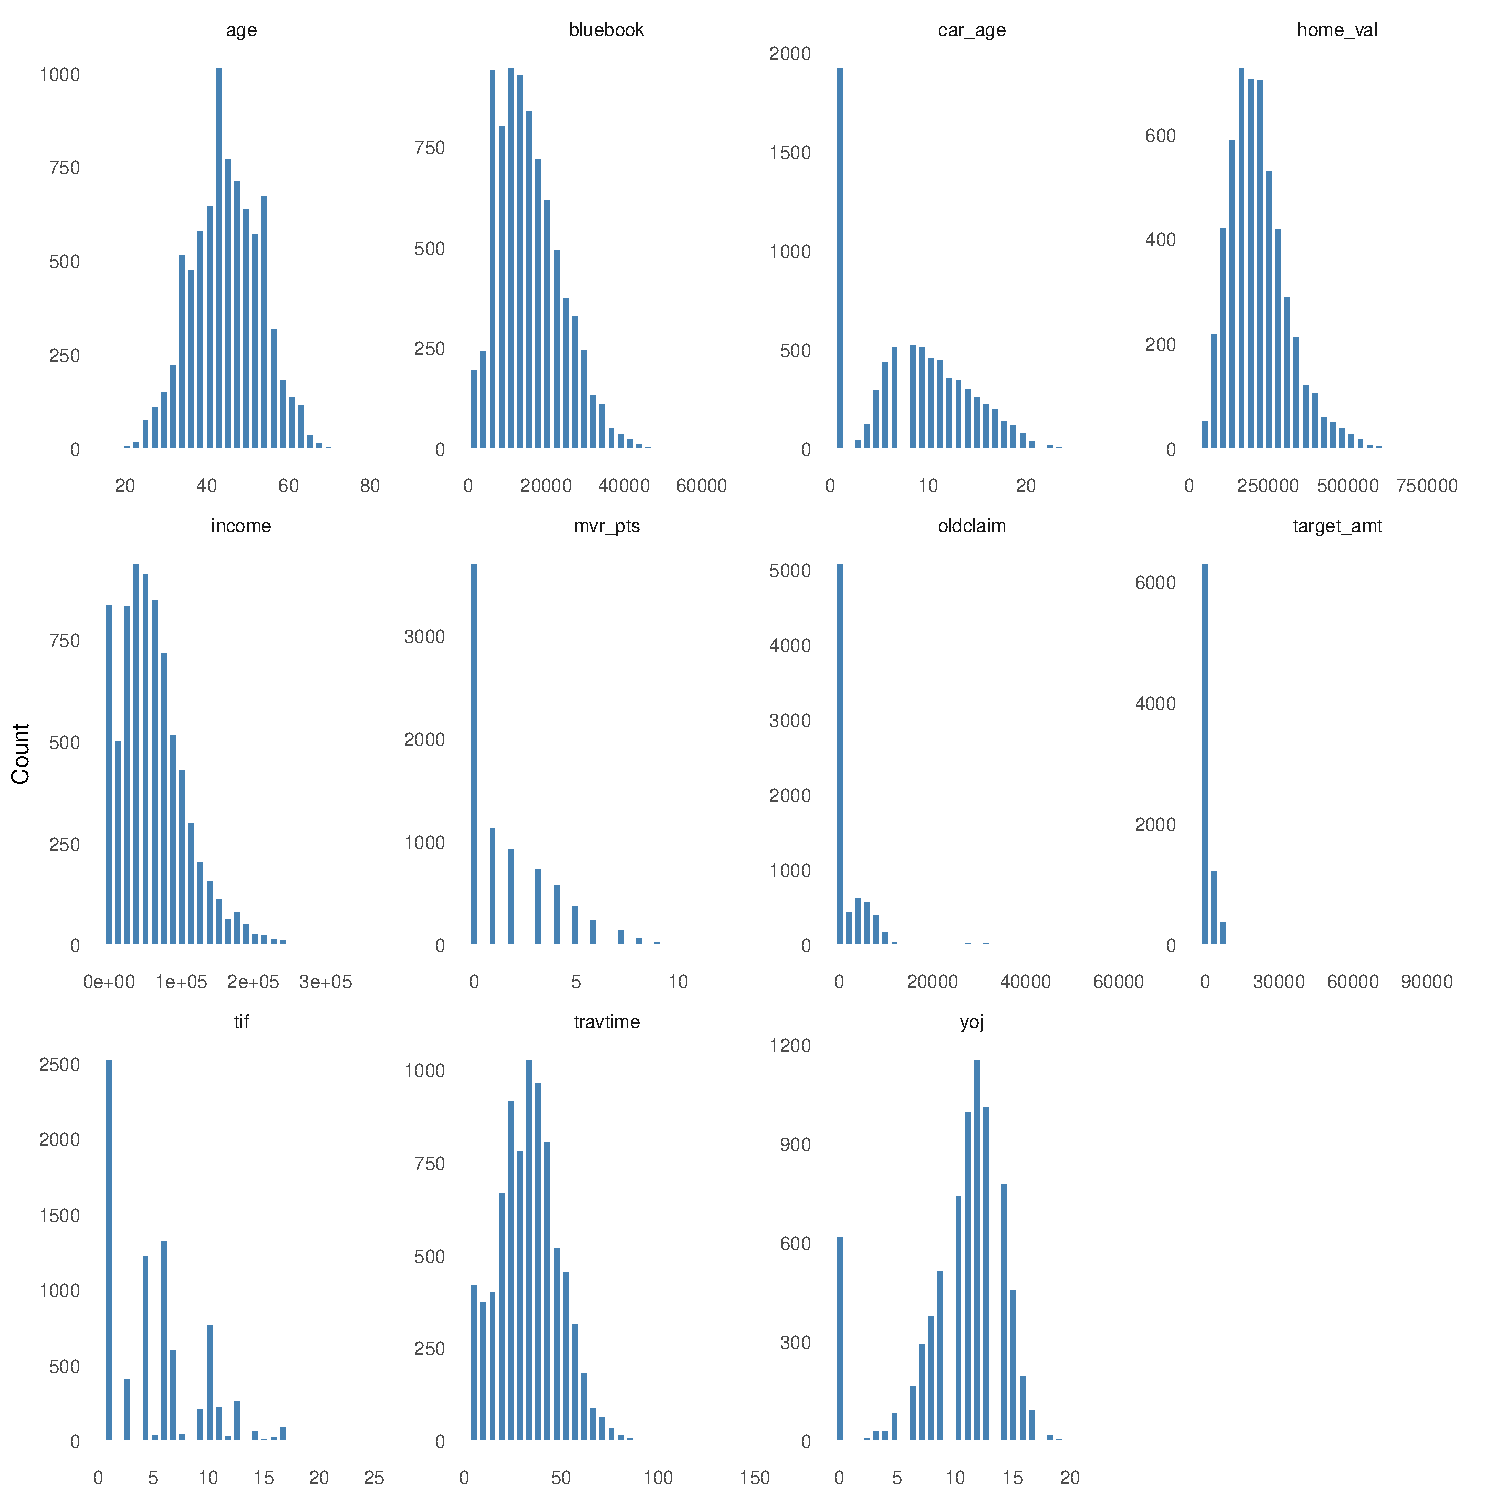
\includegraphics[keepaspectratio]{HW-4_files/figure-pdf/fig-distributions-1.pdf}}

}

\caption{\label{fig-distributions}Distribution of continuous variables
in the training dataset.}

\end{figure}%

There are many 1-year old cars in the dataset, showing a high spike at 1
in the \texttt{car\_age} variable. Dollar amounts such as
\texttt{bluebook}, \texttt{home\_val}, \texttt{income}, and
\texttt{target\_amt} are right-skewed, which is expected for financial
variables. The same goes for travel time (\texttt{travtime}). Most
people have no motor vehicle record points (\texttt{mvr\_pts}) or claims
in the past 5 years (\texttt{oldclaim}), which is expected for a general
population. Years on the job (\texttt{yoj}) is almost normally
distributed, but has a spike at 0, which may represent people who are
unemployed or have been on the job for less than a year.

\section{Data Preparation}\label{data-preparation}

The goal of this section is to prepare the insurance training and
evaluation data for modeling. The assignment requires transformations of
the original variables or the creation of new variables when useful. In
this dataset, preparation included missing value treatment, missingness
flags, mathematical transformations, and derived variables.

\begin{Shaded}
\begin{Highlighting}[]
\CommentTok{\# Identify numeric predictor variables}
\NormalTok{numeric\_vars }\OtherTok{\textless{}{-}}\NormalTok{ insurance\_train\_dummies }\SpecialCharTok{|\textgreater{}}
  \FunctionTok{select}\NormalTok{(}\FunctionTok{where}\NormalTok{(is.numeric)) }\SpecialCharTok{|\textgreater{}}
  \FunctionTok{select}\NormalTok{(}\SpecialCharTok{{-}}\NormalTok{target\_flag, }\SpecialCharTok{{-}}\NormalTok{target\_amt) }\SpecialCharTok{|\textgreater{}}
  \FunctionTok{names}\NormalTok{()}

\CommentTok{\# Create missingness flags before imputation}
\NormalTok{insurance\_train\_prepared }\OtherTok{\textless{}{-}}\NormalTok{ insurance\_train\_dummies }\SpecialCharTok{|\textgreater{}}
  \FunctionTok{mutate}\NormalTok{(}
    \AttributeTok{age\_missing =} \FunctionTok{ifelse}\NormalTok{(}\FunctionTok{is.na}\NormalTok{(age), }\DecValTok{1}\NormalTok{, }\DecValTok{0}\NormalTok{),}
    \AttributeTok{car\_age\_missing =} \FunctionTok{ifelse}\NormalTok{(}\FunctionTok{is.na}\NormalTok{(car\_age), }\DecValTok{1}\NormalTok{, }\DecValTok{0}\NormalTok{),}
    \AttributeTok{home\_val\_missing =} \FunctionTok{ifelse}\NormalTok{(}\FunctionTok{is.na}\NormalTok{(home\_val), }\DecValTok{1}\NormalTok{, }\DecValTok{0}\NormalTok{),}
    \AttributeTok{income\_missing =} \FunctionTok{ifelse}\NormalTok{(}\FunctionTok{is.na}\NormalTok{(income), }\DecValTok{1}\NormalTok{, }\DecValTok{0}\NormalTok{),}
    \AttributeTok{yoj\_missing =} \FunctionTok{ifelse}\NormalTok{(}\FunctionTok{is.na}\NormalTok{(yoj), }\DecValTok{1}\NormalTok{, }\DecValTok{0}\NormalTok{)}
\NormalTok{  )}

\NormalTok{insurance\_eval\_prepared }\OtherTok{\textless{}{-}}\NormalTok{ insurance\_eval\_dummies }\SpecialCharTok{|\textgreater{}}
  \FunctionTok{mutate}\NormalTok{(}
    \AttributeTok{age\_missing =} \FunctionTok{ifelse}\NormalTok{(}\FunctionTok{is.na}\NormalTok{(age), }\DecValTok{1}\NormalTok{, }\DecValTok{0}\NormalTok{),}
    \AttributeTok{car\_age\_missing =} \FunctionTok{ifelse}\NormalTok{(}\FunctionTok{is.na}\NormalTok{(car\_age), }\DecValTok{1}\NormalTok{, }\DecValTok{0}\NormalTok{),}
    \AttributeTok{home\_val\_missing =} \FunctionTok{ifelse}\NormalTok{(}\FunctionTok{is.na}\NormalTok{(home\_val), }\DecValTok{1}\NormalTok{, }\DecValTok{0}\NormalTok{),}
    \AttributeTok{income\_missing =} \FunctionTok{ifelse}\NormalTok{(}\FunctionTok{is.na}\NormalTok{(income), }\DecValTok{1}\NormalTok{, }\DecValTok{0}\NormalTok{),}
    \AttributeTok{yoj\_missing =} \FunctionTok{ifelse}\NormalTok{(}\FunctionTok{is.na}\NormalTok{(yoj), }\DecValTok{1}\NormalTok{, }\DecValTok{0}\NormalTok{)}
\NormalTok{  )}

\CommentTok{\# Median imputation using training medians}
\ControlFlowTok{for}\NormalTok{ (v }\ControlFlowTok{in}\NormalTok{ numeric\_vars) \{}
\NormalTok{  med\_val }\OtherTok{\textless{}{-}} \FunctionTok{median}\NormalTok{(insurance\_train\_prepared[[v]], }\AttributeTok{na.rm =} \ConstantTok{TRUE}\NormalTok{)}

\NormalTok{  insurance\_train\_prepared[[v]][}\FunctionTok{is.na}\NormalTok{(insurance\_train\_prepared[[v]])] }\OtherTok{\textless{}{-}}\NormalTok{ med\_val}
\NormalTok{  insurance\_eval\_prepared[[v]][}\FunctionTok{is.na}\NormalTok{(insurance\_eval\_prepared[[v]])] }\OtherTok{\textless{}{-}}\NormalTok{ med\_val}
\NormalTok{\}}

\CommentTok{\# Create transformed and engineered variables}
\NormalTok{insurance\_train\_prepared }\OtherTok{\textless{}{-}}\NormalTok{ insurance\_train\_prepared }\SpecialCharTok{|\textgreater{}}
  \FunctionTok{mutate}\NormalTok{(}
    \AttributeTok{log\_income =} \FunctionTok{log1p}\NormalTok{(income),}
    \AttributeTok{log\_home\_val =} \FunctionTok{log1p}\NormalTok{(home\_val),}
    \AttributeTok{log\_bluebook =} \FunctionTok{log1p}\NormalTok{(bluebook),}
    \AttributeTok{log\_oldclaim =} \FunctionTok{log1p}\NormalTok{(oldclaim),}
    \AttributeTok{log\_travtime =} \FunctionTok{log1p}\NormalTok{(travtime),}

    \AttributeTok{claim\_rate =}\NormalTok{ oldclaim }\SpecialCharTok{/}\NormalTok{ (clm\_freq }\SpecialCharTok{+} \DecValTok{1}\NormalTok{),}
    \AttributeTok{car\_value\_age\_ratio =}\NormalTok{ bluebook }\SpecialCharTok{/}\NormalTok{ (car\_age }\SpecialCharTok{+} \DecValTok{1}\NormalTok{),}
    \AttributeTok{risk\_points\_claims =}\NormalTok{ mvr\_pts }\SpecialCharTok{+}\NormalTok{ clm\_freq,}

    \AttributeTok{age\_bucket =} \FunctionTok{case\_when}\NormalTok{(}
\NormalTok{      age }\SpecialCharTok{\textless{}} \DecValTok{25} \SpecialCharTok{\textasciitilde{}} \StringTok{"young\_driver"}\NormalTok{,}
\NormalTok{      age }\SpecialCharTok{\textgreater{}=} \DecValTok{25} \SpecialCharTok{\&}\NormalTok{ age }\SpecialCharTok{\textless{}} \DecValTok{60} \SpecialCharTok{\textasciitilde{}} \StringTok{"adult\_driver"}\NormalTok{,}
\NormalTok{      age }\SpecialCharTok{\textgreater{}=} \DecValTok{60} \SpecialCharTok{\textasciitilde{}} \StringTok{"older\_driver"}\NormalTok{,}
      \ConstantTok{TRUE} \SpecialCharTok{\textasciitilde{}} \StringTok{"unknown"}
\NormalTok{    )}
\NormalTok{  )}

\NormalTok{insurance\_eval\_prepared }\OtherTok{\textless{}{-}}\NormalTok{ insurance\_eval\_prepared }\SpecialCharTok{|\textgreater{}}
  \FunctionTok{mutate}\NormalTok{(}
    \AttributeTok{log\_income =} \FunctionTok{log1p}\NormalTok{(income),}
    \AttributeTok{log\_home\_val =} \FunctionTok{log1p}\NormalTok{(home\_val),}
    \AttributeTok{log\_bluebook =} \FunctionTok{log1p}\NormalTok{(bluebook),}
    \AttributeTok{log\_oldclaim =} \FunctionTok{log1p}\NormalTok{(oldclaim),}
    \AttributeTok{log\_travtime =} \FunctionTok{log1p}\NormalTok{(travtime),}

    \AttributeTok{claim\_rate =}\NormalTok{ oldclaim }\SpecialCharTok{/}\NormalTok{ (clm\_freq }\SpecialCharTok{+} \DecValTok{1}\NormalTok{),}
    \AttributeTok{car\_value\_age\_ratio =}\NormalTok{ bluebook }\SpecialCharTok{/}\NormalTok{ (car\_age }\SpecialCharTok{+} \DecValTok{1}\NormalTok{),}
    \AttributeTok{risk\_points\_claims =}\NormalTok{ mvr\_pts }\SpecialCharTok{+}\NormalTok{ clm\_freq,}

    \AttributeTok{age\_bucket =} \FunctionTok{case\_when}\NormalTok{(}
\NormalTok{      age }\SpecialCharTok{\textless{}} \DecValTok{25} \SpecialCharTok{\textasciitilde{}} \StringTok{"young\_driver"}\NormalTok{,}
\NormalTok{      age }\SpecialCharTok{\textgreater{}=} \DecValTok{25} \SpecialCharTok{\&}\NormalTok{ age }\SpecialCharTok{\textless{}} \DecValTok{60} \SpecialCharTok{\textasciitilde{}} \StringTok{"adult\_driver"}\NormalTok{,}
\NormalTok{      age }\SpecialCharTok{\textgreater{}=} \DecValTok{60} \SpecialCharTok{\textasciitilde{}} \StringTok{"older\_driver"}\NormalTok{,}
      \ConstantTok{TRUE} \SpecialCharTok{\textasciitilde{}} \StringTok{"unknown"}
\NormalTok{    )}
\NormalTok{  )}

\CommentTok{\# Convert age bucket into dummy variables}
\NormalTok{insurance\_train\_prepared }\OtherTok{\textless{}{-}}\NormalTok{ fastDummies}\SpecialCharTok{::}\FunctionTok{dummy\_cols}\NormalTok{(}
\NormalTok{  insurance\_train\_prepared,}
  \AttributeTok{select\_columns =} \StringTok{"age\_bucket"}\NormalTok{,}
  \AttributeTok{remove\_selected\_columns =} \ConstantTok{TRUE}\NormalTok{,}
  \AttributeTok{remove\_first\_dummy =} \ConstantTok{TRUE}
\NormalTok{)}

\NormalTok{insurance\_eval\_prepared }\OtherTok{\textless{}{-}}\NormalTok{ fastDummies}\SpecialCharTok{::}\FunctionTok{dummy\_cols}\NormalTok{(}
\NormalTok{  insurance\_eval\_prepared,}
  \AttributeTok{select\_columns =} \StringTok{"age\_bucket"}\NormalTok{,}
  \AttributeTok{remove\_selected\_columns =} \ConstantTok{TRUE}\NormalTok{,}
  \AttributeTok{remove\_first\_dummy =} \ConstantTok{TRUE}
\NormalTok{)}

\CommentTok{\# Confirm no missing values remain}
\FunctionTok{sum}\NormalTok{(}\FunctionTok{is.na}\NormalTok{(insurance\_train\_prepared))}
\end{Highlighting}
\end{Shaded}

\begin{verbatim}
[1] 0
\end{verbatim}

\begin{Shaded}
\begin{Highlighting}[]
\FunctionTok{sum}\NormalTok{(}\FunctionTok{is.na}\NormalTok{(insurance\_eval\_prepared))}
\end{Highlighting}
\end{Shaded}

\begin{verbatim}
[1] 4282
\end{verbatim}

\subsection{Data Splits}\label{data-splits}

First, we will split our dataset into a training and testing set. We
will use the training set to build our models and the testing set to
evaluate their performance. The training set will be used to fit the
models, while the testing set will be used to assess how well the models
generalize to new data.

\begin{Shaded}
\begin{Highlighting}[]
\FunctionTok{set.seed}\NormalTok{(}\DecValTok{19940211}\NormalTok{)}
\NormalTok{train\_indices }\OtherTok{\textless{}{-}} \FunctionTok{sample}\NormalTok{(}\FunctionTok{nrow}\NormalTok{(insurance\_train\_prepared), }\AttributeTok{size =} \FloatTok{0.8} \SpecialCharTok{*} \FunctionTok{nrow}\NormalTok{(insurance\_train\_prepared))}
\NormalTok{insurance\_train\_split }\OtherTok{\textless{}{-}}\NormalTok{ insurance\_train\_prepared[train\_indices, ]}
\NormalTok{insurance\_test\_split }\OtherTok{\textless{}{-}}\NormalTok{ insurance\_train\_prepared[}\SpecialCharTok{{-}}\NormalTok{train\_indices, ]}
\end{Highlighting}
\end{Shaded}

\subsubsection{Linearity Assumption
Summary}\label{linearity-assumption-summary}

The results above indicate that the assumption of linearity is satisfied
for all independent variables. However, several were flagged as being
unlikely to have predictive value in a multivariate linear model.

\section{Check assumptions for binary logistic
regression}\label{check-assumptions-for-binary-logistic-regression}

\begin{enumerate}
\def\labelenumi{\arabic{enumi}.}
\tightlist
\item
  Binary Outcome
\end{enumerate}

\begin{Shaded}
\begin{Highlighting}[]
\CommentTok{\# Confirming that the target is binary}
\NormalTok{crime\_clean }\SpecialCharTok{|\textgreater{}}
    \FunctionTok{count}\NormalTok{(target) }\SpecialCharTok{|\textgreater{}}
    \FunctionTok{mutate}\NormalTok{(}\AttributeTok{prop =}\NormalTok{ n }\SpecialCharTok{/} \FunctionTok{sum}\NormalTok{(n))}
\end{Highlighting}
\end{Shaded}

The response variable ``target'' is confirmed to be a binary, therefore
it takes two values ( 0: crime rate below the median) and (1: crime rate
above the median). In the 466 neighborhoods in training data set 237
(50.9\%) fall in the class of low crime and 228 (49.1)\% are in the high
crime neighborhood. There is no class imbalance, due to the near equal
split meaning there is unlikely to be bias towards one class.

\begin{enumerate}
\def\labelenumi{\arabic{enumi}.}
\setcounter{enumi}{1}
\tightlist
\item
  Independence of Observations
\end{enumerate}

\vspace{0.5em}

Each record in the dataset represents a distinct neighborhood, and there
is no repeated-measures or clustered structure in the data. Therefore,
the independence of observations assumption is satisfied by design and
requires no further adjustment.

\begin{enumerate}
\def\labelenumi{\arabic{enumi}.}
\setcounter{enumi}{2}
\tightlist
\item
  No Multicollinearity (VIF Check)
\end{enumerate}

\begin{Shaded}
\begin{Highlighting}[]
\FunctionTok{library}\NormalTok{(car)}

\CommentTok{\# Fit a reference logistic model with original predictors}
\NormalTok{model\_ref }\OtherTok{\textless{}{-}} \FunctionTok{glm}\NormalTok{(}
\NormalTok{    target }\SpecialCharTok{\textasciitilde{}}\NormalTok{ zn }\SpecialCharTok{+}\NormalTok{ indus }\SpecialCharTok{+}\NormalTok{ chas }\SpecialCharTok{+}\NormalTok{ nox }\SpecialCharTok{+}\NormalTok{ rm }\SpecialCharTok{+}\NormalTok{ age }\SpecialCharTok{+}\NormalTok{ dis }\SpecialCharTok{+}\NormalTok{ rad }\SpecialCharTok{+}\NormalTok{ tax }\SpecialCharTok{+}\NormalTok{ ptratio}
        \SpecialCharTok{+}\NormalTok{ lstat }\SpecialCharTok{+}\NormalTok{ medv,}
    \AttributeTok{data =}\NormalTok{ crime\_clean, }\AttributeTok{family =}\NormalTok{ binomial}
\NormalTok{)}

\CommentTok{\# Compute VIF}
\NormalTok{vif\_vals }\OtherTok{\textless{}{-}} \FunctionTok{vif}\NormalTok{(model\_ref) }\SpecialCharTok{|\textgreater{}}
    \FunctionTok{as.data.frame}\NormalTok{() }\SpecialCharTok{|\textgreater{}}
    \FunctionTok{rownames\_to\_column}\NormalTok{(}\StringTok{"Variable"}\NormalTok{) }\SpecialCharTok{|\textgreater{}}
    \FunctionTok{rename}\NormalTok{(}\AttributeTok{VIF =} \DecValTok{2}\NormalTok{) }\SpecialCharTok{|\textgreater{}}
    \FunctionTok{arrange}\NormalTok{(}\FunctionTok{desc}\NormalTok{(VIF))}

\NormalTok{vif\_vals }\SpecialCharTok{|\textgreater{}}\NormalTok{ knitr}\SpecialCharTok{::}\FunctionTok{kable}\NormalTok{(}\AttributeTok{caption =} \StringTok{"Variance Inflation Factors for Reference Model"}\NormalTok{)}
\end{Highlighting}
\end{Shaded}

The VIF values is calculated for all predictors to check for
multicollinearity. A VIF above 10 is considered to be severe, while
between 5 and 10 should warrant caution. None of the variable exceed a
threshold of 10, indicating multicollinearity is not present.The highest
VIF belongs to medv (median home value, VIF = 8.12), followed by rm
(average rooms per dwelling, VIF = 5.81). These two variables are
moderate and do not need requrie any removal. The remaining predictors
fall below 5 and are acceptable levels of multicollinearity. There was
strong pairwise correlation between ``rad'' and ``tax'' in the
exploration section, howevr it is confirmed that multicollinearity does
not exist in the dataset.

\begin{enumerate}
\def\labelenumi{\arabic{enumi}.}
\setcounter{enumi}{3}
\tightlist
\item
  Linearity of Log-Odds (Box-Tidwell Test)
\end{enumerate}

\begin{Shaded}
\begin{Highlighting}[]
\CommentTok{\# Box{-}Tidwell test: add interaction of each continuous predictor with its log}
\CommentTok{\# to test whether the log{-}odds relationship is linear}
\NormalTok{continuous\_vars }\OtherTok{\textless{}{-}} \FunctionTok{c}\NormalTok{(}
    \StringTok{"zn"}\NormalTok{, }\StringTok{"indus"}\NormalTok{, }\StringTok{"nox"}\NormalTok{, }\StringTok{"rm"}\NormalTok{, }\StringTok{"age"}\NormalTok{, }\StringTok{"dis"}\NormalTok{, }\StringTok{"rad"}\NormalTok{, }\StringTok{"tax"}\NormalTok{,}
    \StringTok{"ptratio"}\NormalTok{, }\StringTok{"lstat"}\NormalTok{, }\StringTok{"medv"}
\NormalTok{)}

\CommentTok{\# Create interaction terms x * log(x) for each continuous predictor}
\CommentTok{\# (use log1p to handle zeros)}
\NormalTok{crime\_bt }\OtherTok{\textless{}{-}}\NormalTok{ crime\_clean }\SpecialCharTok{|\textgreater{}}
    \FunctionTok{mutate}\NormalTok{(}\FunctionTok{across}\NormalTok{(}\FunctionTok{all\_of}\NormalTok{(continuous\_vars), }\SpecialCharTok{\textasciitilde{}}\NormalTok{ . }\SpecialCharTok{*} \FunctionTok{log1p}\NormalTok{(.), }\AttributeTok{.names =} \StringTok{"\{.col\}\_logx"}\NormalTok{))}

\NormalTok{bt\_formula }\OtherTok{\textless{}{-}} \FunctionTok{as.formula}\NormalTok{(}\FunctionTok{paste}\NormalTok{(}
    \StringTok{"target \textasciitilde{}"}\NormalTok{,}
    \FunctionTok{paste}\NormalTok{(continuous\_vars, }\AttributeTok{collapse =} \StringTok{" + "}\NormalTok{),}
    \StringTok{"+"}\NormalTok{,}
    \FunctionTok{paste}\NormalTok{(}\FunctionTok{paste0}\NormalTok{(continuous\_vars, }\StringTok{"\_logx"}\NormalTok{), }\AttributeTok{collapse =} \StringTok{" + "}\NormalTok{)}
\NormalTok{))}

\NormalTok{model\_bt }\OtherTok{\textless{}{-}} \FunctionTok{glm}\NormalTok{(bt\_formula, }\AttributeTok{data =}\NormalTok{ crime\_bt, }\AttributeTok{family =}\NormalTok{ binomial)}

\CommentTok{\# Extract p{-}values for the interaction terms only}
\NormalTok{bt\_results }\OtherTok{\textless{}{-}} \FunctionTok{summary}\NormalTok{(model\_bt)}\SpecialCharTok{$}\NormalTok{coefficients }\SpecialCharTok{|\textgreater{}}
    \FunctionTok{as.data.frame}\NormalTok{() }\SpecialCharTok{|\textgreater{}}
    \FunctionTok{rownames\_to\_column}\NormalTok{(}\StringTok{"Term"}\NormalTok{) }\SpecialCharTok{|\textgreater{}}
    \FunctionTok{filter}\NormalTok{(}\FunctionTok{str\_detect}\NormalTok{(Term, }\StringTok{"\_logx"}\NormalTok{)) }\SpecialCharTok{|\textgreater{}}
    \FunctionTok{mutate}\NormalTok{(}
        \AttributeTok{Variable =} \FunctionTok{str\_remove}\NormalTok{(Term, }\StringTok{"\_logx"}\NormalTok{),}
        \AttributeTok{Significant =} \StringTok{\textasciigrave{}}\AttributeTok{Pr(\textgreater{}|z|)}\StringTok{\textasciigrave{}} \SpecialCharTok{\textless{}} \FloatTok{0.05}
\NormalTok{    ) }\SpecialCharTok{|\textgreater{}}
    \FunctionTok{select}\NormalTok{(Variable, Estimate, }\StringTok{\textasciigrave{}}\AttributeTok{Pr(\textgreater{}|z|)}\StringTok{\textasciigrave{}}\NormalTok{, Significant) }\SpecialCharTok{|\textgreater{}}
    \FunctionTok{mutate}\NormalTok{(}\FunctionTok{across}\NormalTok{(}\FunctionTok{where}\NormalTok{(is.numeric), }\SpecialCharTok{\textasciitilde{}} \FunctionTok{signif}\NormalTok{(., }\DecValTok{3}\NormalTok{)))}

\NormalTok{bt\_results }\SpecialCharTok{|\textgreater{}}\NormalTok{ knitr}\SpecialCharTok{::}\FunctionTok{kable}\NormalTok{(}\AttributeTok{caption =} \StringTok{"Box{-}Tidwell Test for Linearity of Log{-}Odds"}\NormalTok{)}
\end{Highlighting}
\end{Shaded}

The Box-Tidwell test was used to assess whether each continuous
predictor has a linear relationship with the log-odds of the outcome. A
p-value greater than 0.05 violate the assumption. There are three
variables that were flagged as significant:rm (p = 0.003), dis (p
\textless{} 0.001), and tax (p \textless{} 0.001). This indicates that
these predictors do not have strict lienear relationship with log-odds
of high crime. Log transformation were applied to these variables in the
data preparation section in order to be used in the model building. The
remaining eight predictors did not have any evidence of violating the
linearity assumption.

\section{Build models}\label{build-models}

We will build models for two separate outcomes:

\begin{enumerate}
\def\labelenumi{\arabic{enumi}.}
\tightlist
\item
  \textbf{target\_flag} (binary): Whether the person was in a car crash
  (1) or not (0)
\item
  \textbf{target\_amt} (continuous): The amount of money the crash cost
  if it occurs
\end{enumerate}

For each outcome, we compare three models as per the textbook methods: -
Model 1: Full model with all predictors - Model 2: Reduced model
(removing highly correlated or insignificant variables) - Model 3:
Backward stepwise selection model

\subsection{Model 1. Full Logistic and Linear
Models}\label{model-1.-full-logistic-and-linear-models}

As shown below, the most significant predictors for
\texttt{target\_flag} (whether a crash occurred) include variables
related to the driver's profile and history. The AIC for this logistic
model is \texttt{r\textbackslash{}\ AIC(model1\_logistic)}.

Similarly, for \texttt{target\_amt} (cost of crash), the full linear
model identifies significant predictors. The R-squared for this model is
\texttt{r\textbackslash{}\ summary(model1\_linear)\$r.squared}.

\begin{Shaded}
\begin{Highlighting}[]
\CommentTok{\# Model 1: Full Logistic Model (target\_flag)}
\CommentTok{\# This model uses all available numeric predictors}
\NormalTok{model1\_logistic }\OtherTok{\textless{}{-}} \FunctionTok{glm}\NormalTok{(}
    \AttributeTok{formula =}\NormalTok{ target\_flag }\SpecialCharTok{\textasciitilde{}}\NormalTok{ .,}
    \AttributeTok{data =}\NormalTok{ insurance\_train\_split }\SpecialCharTok{|\textgreater{}} \FunctionTok{select}\NormalTok{(}\SpecialCharTok{{-}}\NormalTok{target\_amt),}
    \AttributeTok{family =}\NormalTok{ binomial}
\NormalTok{)}

\FunctionTok{cat}\NormalTok{(}\StringTok{"}\SpecialCharTok{\textbackslash{}n}\StringTok{=== Full Logistic Model Summary ===}\SpecialCharTok{\textbackslash{}n}\StringTok{"}\NormalTok{)}
\end{Highlighting}
\end{Shaded}

\begin{verbatim}

=== Full Logistic Model Summary ===
\end{verbatim}

\begin{Shaded}
\begin{Highlighting}[]
\FunctionTok{summary}\NormalTok{(model1\_logistic)}
\end{Highlighting}
\end{Shaded}

\begin{verbatim}

Call:
glm(formula = target_flag ~ ., family = binomial, data = select(insurance_train_split, 
    -target_amt))

Coefficients: (1 not defined because of singularities)
                          Estimate Std. Error z value Pr(>|z|)    
(Intercept)              7.944e+00  4.389e+00   1.810 0.070287 .  
kidsdriv                 4.407e-01  6.883e-02   6.403 1.52e-10 ***
age                     -7.728e-03  5.236e-03  -1.476 0.139948    
homekids                 6.359e-03  4.222e-02   0.151 0.880264    
yoj                      1.437e-02  1.258e-02   1.142 0.253363    
income                  -1.855e-06  1.521e-06  -1.220 0.222471    
home_val                 1.026e-06  1.940e-06   0.529 0.597085    
travtime                 9.614e-03  6.062e-03   1.586 0.112719    
bluebook                 5.090e-06  1.249e-05   0.407 0.683678    
tif                     -5.336e-02  8.322e-03  -6.411 1.44e-10 ***
oldclaim                -2.687e-05  1.382e-05  -1.945 0.051786 .  
clm_freq                 1.617e-02  6.380e-02   0.253 0.799915    
mvr_pts                  9.445e-02  1.587e-02   5.952 2.65e-09 ***
car_age                  4.851e-03  1.200e-02   0.404 0.685993    
parent1_yes              4.088e-01  1.238e-01   3.301 0.000962 ***
mstatus_z_no             4.909e-01  9.584e-02   5.122 3.02e-07 ***
female                  -1.415e-01  1.278e-01  -1.108 0.268011    
education_bachelors     -3.574e-01  1.326e-01  -2.694 0.007049 ** 
education_masters       -3.316e-01  2.080e-01  -1.594 0.110934    
education_phd           -4.985e-01  2.513e-01  -1.984 0.047281 *  
education_high_school    5.154e-02  1.091e-01   0.473 0.636525    
job_doctor              -7.560e-01  3.343e-01  -2.261 0.023736 *  
job_home_maker          -5.309e-01  1.844e-01  -2.879 0.003991 ** 
job_lawyer              -3.305e-01  2.103e-01  -1.572 0.116049    
job_manager             -9.606e-01  1.614e-01  -5.951 2.67e-09 ***
job_professional        -2.989e-01  1.404e-01  -2.129 0.033285 *  
job_student             -5.214e-01  1.722e-01  -3.028 0.002464 ** 
job_blue_collar         -1.258e-01  1.213e-01  -1.037 0.299751    
job_na                  -3.484e-01  2.242e-01  -1.554 0.120120    
car_use_private         -7.139e-01  1.041e-01  -6.855 7.12e-12 ***
car_type_panel_truck     5.357e-01  1.873e-01   2.860 0.004237 ** 
car_type_pickup          5.797e-01  1.139e-01   5.091 3.57e-07 ***
car_type_sports_car      9.700e-01  1.497e-01   6.482 9.07e-11 ***
car_type_van             6.665e-01  1.439e-01   4.633 3.60e-06 ***
car_type_suv             7.805e-01  1.276e-01   6.118 9.46e-10 ***
red_car_yes             -1.006e-01  9.876e-02  -1.019 0.308307    
revoked_yes              9.370e-01  1.048e-01   8.941  < 2e-16 ***
urbanicity_highly_rural -2.353e+00  1.278e-01 -18.416  < 2e-16 ***
age_missing              1.978e+00  1.230e+00   1.608 0.107754    
car_age_missing          1.679e-01  1.368e-01   1.227 0.219674    
home_val_missing         3.324e-01  9.554e-02   3.480 0.000502 ***
income_missing           1.810e-02  1.500e-01   0.121 0.903968    
yoj_missing              6.266e-02  1.439e-01   0.435 0.663252    
log_income              -7.355e-02  2.267e-02  -3.244 0.001177 ** 
log_home_val            -4.556e-01  3.831e-01  -1.189 0.234347    
log_bluebook            -4.049e-01  1.392e-01  -2.908 0.003633 ** 
log_oldclaim             8.193e-02  1.980e-02   4.138 3.51e-05 ***
log_travtime             2.118e-01  1.727e-01   1.226 0.220103    
claim_rate              -3.106e-06  3.730e-05  -0.083 0.933638    
car_value_age_ratio      1.851e-05  1.850e-05   1.000 0.317098    
risk_points_claims              NA         NA      NA       NA    
age_bucket_older_driver  7.900e-01  1.886e-01   4.190 2.79e-05 ***
age_bucket_young_driver  4.971e-01  3.333e-01   1.492 0.135820    
---
Signif. codes:  0 '***' 0.001 '**' 0.01 '*' 0.05 '.' 0.1 ' ' 1

(Dispersion parameter for binomial family taken to be 1)

    Null deviance: 7531.0  on 6527  degrees of freedom
Residual deviance: 5748.1  on 6476  degrees of freedom
AIC: 5852.1

Number of Fisher Scoring iterations: 5
\end{verbatim}

\begin{Shaded}
\begin{Highlighting}[]
\CommentTok{\# Model 1: Full Linear Model (target\_amt)}
\CommentTok{\# This model uses all available numeric predictors}
\NormalTok{model1\_linear }\OtherTok{\textless{}{-}} \FunctionTok{lm}\NormalTok{(}
    \AttributeTok{formula =}\NormalTok{ target\_amt }\SpecialCharTok{\textasciitilde{}}\NormalTok{ .,}
    \AttributeTok{data =}\NormalTok{ insurance\_train\_split }\SpecialCharTok{|\textgreater{}} \FunctionTok{select}\NormalTok{(}\SpecialCharTok{{-}}\NormalTok{target\_flag)}
\NormalTok{)}

\FunctionTok{cat}\NormalTok{(}\StringTok{"}\SpecialCharTok{\textbackslash{}n}\StringTok{=== Full Linear Model Summary ===}\SpecialCharTok{\textbackslash{}n}\StringTok{"}\NormalTok{)}
\end{Highlighting}
\end{Shaded}

\begin{verbatim}

=== Full Linear Model Summary ===
\end{verbatim}

\begin{Shaded}
\begin{Highlighting}[]
\FunctionTok{summary}\NormalTok{(model1\_linear)}
\end{Highlighting}
\end{Shaded}

\begin{verbatim}

Call:
lm(formula = target_amt ~ ., data = select(insurance_train_split, 
    -target_flag))

Residuals:
   Min     1Q Median     3Q    Max 
 -5476  -1694   -760    387 103433 

Coefficients: (1 not defined because of singularities)
                          Estimate Std. Error t value Pr(>|t|)    
(Intercept)              9.078e+02  7.454e+03   0.122  0.90307    
kidsdriv                 3.108e+02  1.287e+02   2.414  0.01579 *  
age                     -1.282e-01  9.262e+00  -0.014  0.98896    
homekids                 3.280e+01  7.557e+01   0.434  0.66433    
yoj                     -1.116e+00  2.189e+01  -0.051  0.95936    
income                  -2.254e-03  2.672e-03  -0.843  0.39899    
home_val                -6.342e-04  3.161e-03  -0.201  0.84098    
travtime                 4.353e+00  1.018e+01   0.427  0.66908    
bluebook                 9.426e-04  2.091e-02   0.045  0.96405    
tif                     -4.269e+01  1.400e+01  -3.049  0.00230 ** 
oldclaim                -6.465e-02  2.699e-02  -2.396  0.01662 *  
clm_freq                 1.338e+02  1.288e+02   1.038  0.29910    
mvr_pts                  1.633e+02  3.062e+01   5.333 9.97e-08 ***
car_age                 -1.753e+01  2.066e+01  -0.848  0.39626    
parent1_yes              5.603e+02  2.313e+02   2.422  0.01545 *  
mstatus_z_no             5.819e+02  1.679e+02   3.467  0.00053 ***
female                  -3.282e+02  2.135e+02  -1.537  0.12437    
education_bachelors     -2.888e+02  2.391e+02  -1.208  0.22723    
education_masters        3.296e+00  3.498e+02   0.009  0.99248    
education_phd           -2.056e+02  4.151e+02  -0.495  0.62046    
education_high_school   -1.813e+02  1.997e+02  -0.908  0.36405    
job_doctor              -9.151e+02  5.033e+02  -1.818  0.06908 .  
job_home_maker          -4.712e+02  3.171e+02  -1.486  0.13727    
job_lawyer              -4.518e+02  3.503e+02  -1.290  0.19716    
job_manager             -1.158e+03  2.726e+02  -4.247 2.20e-05 ***
job_professional        -1.423e+02  2.485e+02  -0.573  0.56696    
job_student             -4.002e+02  3.120e+02  -1.283  0.19962    
job_blue_collar         -8.843e+01  2.221e+02  -0.398  0.69060    
job_na                  -7.612e+02  3.922e+02  -1.941  0.05235 .  
car_use_private         -8.037e+02  1.889e+02  -4.255 2.12e-05 ***
car_type_panel_truck     2.656e+02  3.251e+02   0.817  0.41401    
car_type_pickup          2.608e+02  1.948e+02   1.339  0.18074    
car_type_sports_car      1.009e+03  2.553e+02   3.952 7.85e-05 ***
car_type_van             5.800e+02  2.449e+02   2.369  0.01787 *  
car_type_suv             6.435e+02  2.084e+02   3.088  0.00202 ** 
red_car_yes             -8.997e+01  1.724e+02  -0.522  0.60185    
revoked_yes              5.471e+02  2.003e+02   2.731  0.00633 ** 
urbanicity_highly_rural -1.623e+03  1.617e+02 -10.038  < 2e-16 ***
age_missing              1.162e+03  2.095e+03   0.555  0.57892    
car_age_missing          7.637e+01  2.433e+02   0.314  0.75362    
home_val_missing         1.516e+02  1.741e+02   0.871  0.38383    
income_missing           1.257e+02  2.608e+02   0.482  0.62983    
yoj_missing              3.243e+02  2.523e+02   1.285  0.19869    
log_income              -3.847e+01  4.027e+01  -0.955  0.33946    
log_home_val            -1.993e+01  6.518e+02  -0.031  0.97561    
log_bluebook             1.353e+02  2.453e+02   0.551  0.58139    
log_oldclaim             2.420e+01  3.927e+01   0.616  0.53773    
log_travtime             1.811e+02  2.828e+02   0.640  0.52189    
claim_rate               1.335e-01  7.295e-02   1.830  0.06727 .  
car_value_age_ratio      1.344e-02  3.263e-02   0.412  0.68031    
risk_points_claims              NA         NA      NA       NA    
age_bucket_older_driver  5.248e+02  3.444e+02   1.524  0.12758    
age_bucket_young_driver  3.244e+02  6.563e+02   0.494  0.62111    
---
Signif. codes:  0 '***' 0.001 '**' 0.01 '*' 0.05 '.' 0.1 ' ' 1

Residual standard error: 4643 on 6476 degrees of freedom
Multiple R-squared:  0.0709,    Adjusted R-squared:  0.06359 
F-statistic:  9.69 on 51 and 6476 DF,  p-value: < 2.2e-16
\end{verbatim}

\subsection{Model 2. Reduced Models (Addressing
Multicollinearity)}\label{model-2.-reduced-models-addressing-multicollinearity}

In the Data Exploration section, we identified several variables with
high correlations. For the reduced models, we remove highly correlated
predictors while retaining theoretically important ones.

The AIC for the reduced logistic model is
\texttt{r\textbackslash{}\ AIC(model2\_logistic)}, and the R-squared for
the reduced linear model is
\texttt{r\textbackslash{}\ summary(model2\_linear)\$r.squared}.

\begin{Shaded}
\begin{Highlighting}[]
\CommentTok{\# Model 2: Reduced Logistic Model}
\CommentTok{\# Keep only important predictors based on correlation analysis}
\NormalTok{reduced\_vars }\OtherTok{\textless{}{-}} \FunctionTok{c}\NormalTok{(}\StringTok{"kidsdriv"}\NormalTok{, }\StringTok{"age"}\NormalTok{, }\StringTok{"homekids"}\NormalTok{, }\StringTok{"yoj"}\NormalTok{, }\StringTok{"income"}\NormalTok{, }\StringTok{"home\_val"}\NormalTok{,}
                  \StringTok{"travtime"}\NormalTok{, }\StringTok{"bluebook"}\NormalTok{, }\StringTok{"tif"}\NormalTok{, }\StringTok{"oldclaim"}\NormalTok{, }\StringTok{"clm\_freq"}\NormalTok{, }\StringTok{"mvr\_pts"}\NormalTok{, }\StringTok{"car\_age"}\NormalTok{)}

\NormalTok{model2\_logistic }\OtherTok{\textless{}{-}} \FunctionTok{glm}\NormalTok{(}
    \AttributeTok{formula =} \FunctionTok{as.formula}\NormalTok{(}\FunctionTok{paste}\NormalTok{(}\StringTok{"target\_flag \textasciitilde{}"}\NormalTok{, }\FunctionTok{paste}\NormalTok{(reduced\_vars, }\AttributeTok{collapse =} \StringTok{"+"}\NormalTok{))),}
    \AttributeTok{data =}\NormalTok{ insurance\_train\_split,}
    \AttributeTok{family =}\NormalTok{ binomial}
\NormalTok{)}

\FunctionTok{cat}\NormalTok{(}\StringTok{"}\SpecialCharTok{\textbackslash{}n}\StringTok{=== Reduced Logistic Model Summary ===}\SpecialCharTok{\textbackslash{}n}\StringTok{"}\NormalTok{)}
\end{Highlighting}
\end{Shaded}

\begin{verbatim}

=== Reduced Logistic Model Summary ===
\end{verbatim}

\begin{Shaded}
\begin{Highlighting}[]
\FunctionTok{summary}\NormalTok{(model2\_logistic)}
\end{Highlighting}
\end{Shaded}

\begin{verbatim}

Call:
glm(formula = as.formula(paste("target_flag ~", paste(reduced_vars, 
    collapse = "+"))), family = binomial, data = insurance_train_split)

Coefficients:
              Estimate Std. Error z value Pr(>|z|)    
(Intercept) -4.658e-01  2.236e-01  -2.083 0.037259 *  
kidsdriv     2.977e-01  6.039e-02   4.930 8.23e-07 ***
age         -8.546e-03  3.994e-03  -2.140 0.032383 *  
homekids     8.324e-02  3.304e-02   2.519 0.011754 *  
yoj         -1.752e-02  7.679e-03  -2.281 0.022524 *  
income      -3.230e-06  1.133e-06  -2.851 0.004353 ** 
home_val    -7.670e-07  6.134e-07  -1.250 0.211143    
travtime     8.276e-03  1.848e-03   4.478 7.52e-06 ***
bluebook    -1.400e-05  4.096e-06  -3.419 0.000629 ***
tif         -4.374e-02  7.562e-03  -5.784 7.28e-09 ***
oldclaim     6.127e-06  3.481e-06   1.760 0.078418 .  
clm_freq     2.691e-01  2.868e-02   9.381  < 2e-16 ***
mvr_pts      1.479e-01  1.394e-02  10.616  < 2e-16 ***
car_age     -2.270e-02  6.078e-03  -3.735 0.000188 ***
---
Signif. codes:  0 '***' 0.001 '**' 0.01 '*' 0.05 '.' 0.1 ' ' 1

(Dispersion parameter for binomial family taken to be 1)

    Null deviance: 7531.0  on 6527  degrees of freedom
Residual deviance: 6803.1  on 6514  degrees of freedom
AIC: 6831.1

Number of Fisher Scoring iterations: 4
\end{verbatim}

\begin{Shaded}
\begin{Highlighting}[]
\CommentTok{\# Model 2: Reduced Linear Model}
\NormalTok{model2\_linear }\OtherTok{\textless{}{-}} \FunctionTok{lm}\NormalTok{(}
    \AttributeTok{formula =} \FunctionTok{as.formula}\NormalTok{(}\FunctionTok{paste}\NormalTok{(}\StringTok{"target\_amt \textasciitilde{}"}\NormalTok{, }\FunctionTok{paste}\NormalTok{(reduced\_vars, }\AttributeTok{collapse =} \StringTok{"+"}\NormalTok{))),}
    \AttributeTok{data =}\NormalTok{ insurance\_train\_split}
\NormalTok{)}

\FunctionTok{cat}\NormalTok{(}\StringTok{"}\SpecialCharTok{\textbackslash{}n}\StringTok{=== Reduced Linear Model Summary ===}\SpecialCharTok{\textbackslash{}n}\StringTok{"}\NormalTok{)}
\end{Highlighting}
\end{Shaded}

\begin{verbatim}

=== Reduced Linear Model Summary ===
\end{verbatim}

\begin{Shaded}
\begin{Highlighting}[]
\FunctionTok{summary}\NormalTok{(model2\_linear)}
\end{Highlighting}
\end{Shaded}

\begin{verbatim}

Call:
lm(formula = as.formula(paste("target_amt ~", paste(reduced_vars, 
    collapse = "+"))), data = insurance_train_split)

Residuals:
   Min     1Q Median     3Q    Max 
 -4857  -1565   -968   -200 104001 

Coefficients:
              Estimate Std. Error t value Pr(>|t|)    
(Intercept)  1.517e+03  4.385e+02   3.459 0.000546 ***
kidsdriv     2.569e+02  1.300e+02   1.977 0.048115 *  
age         -4.561e+00  7.936e+00  -0.575 0.565478    
homekids     1.081e+02  6.768e+01   1.598 0.110143    
yoj         -1.700e+01  1.568e+01  -1.084 0.278264    
income      -2.187e-03  2.083e-03  -1.050 0.293755    
home_val    -9.346e-04  1.117e-03  -0.836 0.402940    
travtime     6.382e+00  3.664e+00   1.742 0.081575 .  
bluebook     1.626e-02  7.721e-03   2.106 0.035246 *  
tif         -3.865e+01  1.419e+01  -2.725 0.006450 ** 
oldclaim     5.048e-03  7.649e-03   0.660 0.509260    
clm_freq     2.661e+02  6.168e+01   4.314 1.63e-05 ***
mvr_pts      2.290e+02  2.977e+01   7.692 1.66e-14 ***
car_age     -3.416e+01  1.169e+01  -2.923 0.003475 ** 
---
Signif. codes:  0 '***' 0.001 '**' 0.01 '*' 0.05 '.' 0.1 ' ' 1

Residual standard error: 4725 on 6514 degrees of freedom
Multiple R-squared:  0.03187,   Adjusted R-squared:  0.02994 
F-statistic:  16.5 on 13 and 6514 DF,  p-value: < 2.2e-16
\end{verbatim}

\subsection{Model 3. Backward Stepwise Selection
Models}\label{model-3.-backward-stepwise-selection-models}

For this model, we performed backward stepwise selection from the full
model to identify the most important predictors.

The AIC for the stepwise logistic model is
\texttt{r\textbackslash{}\ AIC(model3\_logistic)}, and the R-squared for
the stepwise linear model is
\texttt{r\textbackslash{}\ summary(model3\_linear)\$r.squared}.

\begin{Shaded}
\begin{Highlighting}[]
\CommentTok{\# Model 3: Backward Stepwise Logistic Model}
\NormalTok{full\_logistic }\OtherTok{\textless{}{-}} \FunctionTok{glm}\NormalTok{(}
    \AttributeTok{formula =}\NormalTok{ target\_flag }\SpecialCharTok{\textasciitilde{}}\NormalTok{ .,}
    \AttributeTok{data =}\NormalTok{ insurance\_train\_split }\SpecialCharTok{|\textgreater{}} \FunctionTok{select}\NormalTok{(}\SpecialCharTok{{-}}\NormalTok{target\_amt),}
    \AttributeTok{family =}\NormalTok{ binomial}
\NormalTok{)}

\NormalTok{model3\_logistic }\OtherTok{\textless{}{-}} \FunctionTok{step}\NormalTok{(full\_logistic, }\AttributeTok{direction =} \StringTok{"backward"}\NormalTok{, }\AttributeTok{trace =} \DecValTok{0}\NormalTok{)}

\FunctionTok{cat}\NormalTok{(}\StringTok{"}\SpecialCharTok{\textbackslash{}n}\StringTok{=== Stepwise Logistic Model Summary ===}\SpecialCharTok{\textbackslash{}n}\StringTok{"}\NormalTok{)}
\end{Highlighting}
\end{Shaded}

\begin{verbatim}

=== Stepwise Logistic Model Summary ===
\end{verbatim}

\begin{Shaded}
\begin{Highlighting}[]
\FunctionTok{summary}\NormalTok{(model3\_logistic)}
\end{Highlighting}
\end{Shaded}

\begin{verbatim}

Call:
glm(formula = target_flag ~ kidsdriv + age + yoj + travtime + 
    tif + oldclaim + mvr_pts + parent1_yes + mstatus_z_no + education_bachelors + 
    education_masters + education_phd + job_doctor + job_home_maker + 
    job_manager + job_professional + job_student + car_use_private + 
    car_type_panel_truck + car_type_pickup + car_type_sports_car + 
    car_type_van + car_type_suv + revoked_yes + urbanicity_highly_rural + 
    age_missing + home_val_missing + log_income + log_home_val + 
    log_bluebook + log_oldclaim + age_bucket_older_driver + age_bucket_young_driver, 
    family = binomial, data = select(insurance_train_split, -target_amt))

Coefficients:
                          Estimate Std. Error z value Pr(>|z|)    
(Intercept)              6.822e+00  1.506e+00   4.529 5.92e-06 ***
kidsdriv                 4.458e-01  6.187e-02   7.205 5.82e-13 ***
age                     -8.248e-03  4.775e-03  -1.728 0.084068 .  
yoj                      1.730e-02  1.193e-02   1.450 0.146972    
travtime                 1.651e-02  2.121e-03   7.785 6.95e-15 ***
tif                     -5.304e-02  8.281e-03  -6.405 1.50e-10 ***
oldclaim                -2.843e-05  5.244e-06  -5.422 5.89e-08 ***
mvr_pts                  9.366e-02  1.582e-02   5.922 3.18e-09 ***
parent1_yes              4.165e-01  1.129e-01   3.688 0.000226 ***
mstatus_z_no             4.828e-01  9.308e-02   5.187 2.14e-07 ***
education_bachelors     -4.629e-01  8.877e-02  -5.215 1.84e-07 ***
education_masters       -6.072e-01  1.005e-01  -6.043 1.51e-09 ***
education_phd           -8.093e-01  1.645e-01  -4.920 8.64e-07 ***
job_doctor              -4.626e-01  2.937e-01  -1.575 0.115221    
job_home_maker          -4.048e-01  1.687e-01  -2.400 0.016413 *  
job_manager             -7.864e-01  1.242e-01  -6.331 2.44e-10 ***
job_professional        -1.566e-01  1.105e-01  -1.418 0.156295    
job_student             -4.131e-01  1.559e-01  -2.650 0.008059 ** 
car_use_private         -6.931e-01  8.427e-02  -8.225  < 2e-16 ***
car_type_panel_truck     6.116e-01  1.552e-01   3.941 8.11e-05 ***
car_type_pickup          5.774e-01  1.109e-01   5.207 1.91e-07 ***
car_type_sports_car      9.063e-01  1.226e-01   7.390 1.47e-13 ***
car_type_van             6.963e-01  1.362e-01   5.114 3.15e-07 ***
car_type_suv             7.223e-01  9.643e-02   7.491 6.85e-14 ***
revoked_yes              9.368e-01  1.044e-01   8.977  < 2e-16 ***
urbanicity_highly_rural -2.344e+00  1.273e-01 -18.412  < 2e-16 ***
age_missing              1.925e+00  1.220e+00   1.577 0.114814    
home_val_missing         3.194e-01  8.744e-02   3.653 0.000259 ***
log_income              -8.588e-02  2.028e-02  -4.234 2.29e-05 ***
log_home_val            -3.525e-01  1.204e-01  -2.929 0.003402 ** 
log_bluebook            -3.376e-01  6.217e-02  -5.430 5.63e-08 ***
log_oldclaim             8.674e-02  1.106e-02   7.846 4.28e-15 ***
age_bucket_older_driver  8.352e-01  1.836e-01   4.550 5.36e-06 ***
age_bucket_young_driver  4.625e-01  3.260e-01   1.419 0.156018    
---
Signif. codes:  0 '***' 0.001 '**' 0.01 '*' 0.05 '.' 0.1 ' ' 1

(Dispersion parameter for binomial family taken to be 1)

    Null deviance: 7531.0  on 6527  degrees of freedom
Residual deviance: 5759.5  on 6494  degrees of freedom
AIC: 5827.5

Number of Fisher Scoring iterations: 5
\end{verbatim}

\begin{Shaded}
\begin{Highlighting}[]
\CommentTok{\# Model 3: Backward Stepwise Linear Model}
\NormalTok{full\_linear }\OtherTok{\textless{}{-}} \FunctionTok{lm}\NormalTok{(}
    \AttributeTok{formula =}\NormalTok{ target\_amt }\SpecialCharTok{\textasciitilde{}}\NormalTok{ .,}
    \AttributeTok{data =}\NormalTok{ insurance\_train\_split }\SpecialCharTok{|\textgreater{}} \FunctionTok{select}\NormalTok{(}\SpecialCharTok{{-}}\NormalTok{target\_flag)}
\NormalTok{)}

\NormalTok{model3\_linear }\OtherTok{\textless{}{-}} \FunctionTok{step}\NormalTok{(full\_linear, }\AttributeTok{direction =} \StringTok{"backward"}\NormalTok{, }\AttributeTok{trace =} \DecValTok{0}\NormalTok{)}

\FunctionTok{cat}\NormalTok{(}\StringTok{"}\SpecialCharTok{\textbackslash{}n}\StringTok{=== Stepwise Linear Model Summary ===}\SpecialCharTok{\textbackslash{}n}\StringTok{"}\NormalTok{)}
\end{Highlighting}
\end{Shaded}

\begin{verbatim}

=== Stepwise Linear Model Summary ===
\end{verbatim}

\begin{Shaded}
\begin{Highlighting}[]
\FunctionTok{summary}\NormalTok{(model3\_linear)}
\end{Highlighting}
\end{Shaded}

\begin{verbatim}

Call:
lm(formula = target_amt ~ kidsdriv + income + tif + oldclaim + 
    clm_freq + mvr_pts + car_age + parent1_yes + mstatus_z_no + 
    female + job_doctor + job_manager + car_use_private + car_type_sports_car + 
    car_type_van + car_type_suv + revoked_yes + urbanicity_highly_rural + 
    log_bluebook + log_travtime + claim_rate + age_bucket_older_driver, 
    data = select(insurance_train_split, -target_flag))

Residuals:
   Min     1Q Median     3Q    Max 
 -5661  -1702   -761    370 103447 

Coefficients:
                          Estimate Std. Error t value Pr(>|t|)    
(Intercept)             -2.607e+02  1.068e+03  -0.244 0.807097    
kidsdriv                 3.507e+02  1.158e+02   3.030 0.002456 ** 
income                  -5.187e-03  1.519e-03  -3.415 0.000641 ***
tif                     -4.178e+01  1.393e+01  -3.000 0.002713 ** 
oldclaim                -7.157e-02  2.564e-02  -2.791 0.005273 ** 
clm_freq                 2.057e+02  6.904e+01   2.979 0.002900 ** 
mvr_pts                  1.723e+02  2.962e+01   5.817 6.28e-09 ***
car_age                 -3.336e+01  1.158e+01  -2.882 0.003970 ** 
parent1_yes              6.379e+02  2.014e+02   3.168 0.001543 ** 
mstatus_z_no             6.349e+02  1.370e+02   4.636 3.62e-06 ***
female                  -2.883e+02  1.702e+02  -1.694 0.090321 .  
job_doctor              -6.149e+02  3.673e+02  -1.674 0.094111 .  
job_manager             -9.248e+02  1.857e+02  -4.980 6.51e-07 ***
car_use_private         -8.311e+02  1.310e+02  -6.343 2.41e-10 ***
car_type_sports_car      9.203e+02  2.393e+02   3.846 0.000121 ***
car_type_van             4.405e+02  2.122e+02   2.076 0.037935 *  
car_type_suv             5.438e+02  1.862e+02   2.920 0.003511 ** 
revoked_yes              5.487e+02  1.982e+02   2.769 0.005640 ** 
urbanicity_highly_rural -1.586e+03  1.569e+02 -10.106  < 2e-16 ***
log_bluebook             1.617e+02  1.073e+02   1.507 0.131773    
log_travtime             2.974e+02  1.013e+02   2.935 0.003347 ** 
claim_rate               1.609e-01  6.197e-02   2.596 0.009440 ** 
age_bucket_older_driver  4.797e+02  3.047e+02   1.575 0.115396    
---
Signif. codes:  0 '***' 0.001 '**' 0.01 '*' 0.05 '.' 0.1 ' ' 1

Residual standard error: 4638 on 6505 degrees of freedom
Multiple R-squared:  0.06857,   Adjusted R-squared:  0.06542 
F-statistic: 21.77 on 22 and 6505 DF,  p-value: < 2.2e-16
\end{verbatim}

Of these three models, the stepwise models have the lowest AIC for
logistic and highest R-squared for linear. In the next section, we will
evaluate the performance of these models to determine which ones are
best for predicting the insurance outcomes.

\section{Select Models}\label{select-models}

We evaluate both logistic and linear regression models using standard
metrics from the textbook methods.

\subsection{Evaluation Metrics
Function}\label{evaluation-metrics-function}

\begin{Shaded}
\begin{Highlighting}[]
\CommentTok{\#\textquotesingle{} Evaluate Logistic Regression Models}
\CommentTok{\#\textquotesingle{} @param model A glm logistic model}
\CommentTok{\#\textquotesingle{} @param model\_name Character name of the model}
\CommentTok{\#\textquotesingle{} @param data Test dataframe}
\CommentTok{\#\textquotesingle{} @param target\_col Name of target column}
\CommentTok{\#\textquotesingle{} @return Tibble with evaluation metrics}
\NormalTok{evaluate\_logistic\_model }\OtherTok{\textless{}{-}} \ControlFlowTok{function}\NormalTok{(model, model\_name, data, }\AttributeTok{target\_col =} \StringTok{"target\_flag"}\NormalTok{) \{}
\NormalTok{    probs }\OtherTok{\textless{}{-}} \FunctionTok{predict}\NormalTok{(model, }\AttributeTok{newdata =}\NormalTok{ data, }\AttributeTok{type =} \StringTok{"response"}\NormalTok{)}
\NormalTok{    preds }\OtherTok{\textless{}{-}} \FunctionTok{factor}\NormalTok{(}\FunctionTok{ifelse}\NormalTok{(probs }\SpecialCharTok{\textgreater{}} \FloatTok{0.5}\NormalTok{, }\DecValTok{1}\NormalTok{, }\DecValTok{0}\NormalTok{), }\AttributeTok{levels =} \FunctionTok{c}\NormalTok{(}\DecValTok{0}\NormalTok{, }\DecValTok{1}\NormalTok{))}
\NormalTok{    actuals }\OtherTok{\textless{}{-}} \FunctionTok{factor}\NormalTok{(data[[target\_col]], }\AttributeTok{levels =} \FunctionTok{c}\NormalTok{(}\DecValTok{0}\NormalTok{, }\DecValTok{1}\NormalTok{))}
    
\NormalTok{    cm }\OtherTok{\textless{}{-}} \FunctionTok{confusionMatrix}\NormalTok{(preds, actuals, }\AttributeTok{positive =} \StringTok{"1"}\NormalTok{)}
\NormalTok{    roc\_obj }\OtherTok{\textless{}{-}} \FunctionTok{roc}\NormalTok{(data[[target\_col]], probs, }\AttributeTok{quiet =} \ConstantTok{TRUE}\NormalTok{)}
\NormalTok{    auc\_val }\OtherTok{\textless{}{-}} \FunctionTok{as.numeric}\NormalTok{(pROC}\SpecialCharTok{::}\FunctionTok{auc}\NormalTok{(roc\_obj))}
    
    \FunctionTok{tibble}\NormalTok{(}
        \AttributeTok{Model =}\NormalTok{ model\_name,}
        \AttributeTok{Deviance =}\NormalTok{ model}\SpecialCharTok{$}\NormalTok{deviance,}
        \AttributeTok{Accuracy =}\NormalTok{ cm}\SpecialCharTok{$}\NormalTok{overall[}\StringTok{"Accuracy"}\NormalTok{],}
        \AttributeTok{Error\_Rate =} \DecValTok{1} \SpecialCharTok{{-}}\NormalTok{ cm}\SpecialCharTok{$}\NormalTok{overall[}\StringTok{"Accuracy"}\NormalTok{],}
        \AttributeTok{Precision =}\NormalTok{ cm}\SpecialCharTok{$}\NormalTok{byClass[}\StringTok{"Precision"}\NormalTok{],}
        \AttributeTok{Sensitivity =}\NormalTok{ cm}\SpecialCharTok{$}\NormalTok{byClass[}\StringTok{"Sensitivity"}\NormalTok{],}
        \AttributeTok{Specificity =}\NormalTok{ cm}\SpecialCharTok{$}\NormalTok{byClass[}\StringTok{"Specificity"}\NormalTok{],}
        \AttributeTok{F1 =}\NormalTok{ cm}\SpecialCharTok{$}\NormalTok{byClass[}\StringTok{"F1"}\NormalTok{],}
        \AttributeTok{AUC =}\NormalTok{ auc\_val,}
        \AttributeTok{AIC =} \FunctionTok{AIC}\NormalTok{(model),}
        \AttributeTok{BIC =} \FunctionTok{BIC}\NormalTok{(model)}
\NormalTok{    )}
\NormalTok{\}}

\CommentTok{\#\textquotesingle{} Evaluate Linear Regression Models}
\CommentTok{\#\textquotesingle{} @param model An lm linear model}
\CommentTok{\#\textquotesingle{} @param model\_name Character name of the model}
\CommentTok{\#\textquotesingle{} @param data Test dataframe}
\CommentTok{\#\textquotesingle{} @param target\_col Name of target column}
\CommentTok{\#\textquotesingle{} @return Tibble with evaluation metrics}
\NormalTok{evaluate\_linear\_model }\OtherTok{\textless{}{-}} \ControlFlowTok{function}\NormalTok{(model, model\_name, data, }\AttributeTok{target\_col =} \StringTok{"target\_amt"}\NormalTok{) \{}
\NormalTok{    preds }\OtherTok{\textless{}{-}} \FunctionTok{predict}\NormalTok{(model, }\AttributeTok{newdata =}\NormalTok{ data)}
\NormalTok{    actuals }\OtherTok{\textless{}{-}}\NormalTok{ data[[target\_col]]}
    
    \CommentTok{\# Calculate metrics}
\NormalTok{    mse }\OtherTok{\textless{}{-}} \FunctionTok{mean}\NormalTok{((actuals }\SpecialCharTok{{-}}\NormalTok{ preds)}\SpecialCharTok{\^{}}\DecValTok{2}\NormalTok{)}
\NormalTok{    rmse }\OtherTok{\textless{}{-}} \FunctionTok{sqrt}\NormalTok{(mse)}
\NormalTok{    mae }\OtherTok{\textless{}{-}} \FunctionTok{mean}\NormalTok{(}\FunctionTok{abs}\NormalTok{(actuals }\SpecialCharTok{{-}}\NormalTok{ preds))}
\NormalTok{    r2 }\OtherTok{\textless{}{-}} \FunctionTok{summary}\NormalTok{(model)}\SpecialCharTok{$}\NormalTok{r.squared}
\NormalTok{    adj\_r2 }\OtherTok{\textless{}{-}} \FunctionTok{summary}\NormalTok{(model)}\SpecialCharTok{$}\NormalTok{adj.r.squared}
    
    \FunctionTok{tibble}\NormalTok{(}
        \AttributeTok{Model =}\NormalTok{ model\_name,}
        \AttributeTok{MSE =}\NormalTok{ mse,}
        \AttributeTok{RMSE =}\NormalTok{ rmse,}
        \AttributeTok{MAE =}\NormalTok{ mae,}
        \AttributeTok{R\_Squared =}\NormalTok{ r2,}
        \AttributeTok{Adj\_R\_Squared =}\NormalTok{ adj\_r2,}
        \AttributeTok{AIC =} \FunctionTok{AIC}\NormalTok{(model),}
        \AttributeTok{BIC =} \FunctionTok{BIC}\NormalTok{(model)}
\NormalTok{    )}
\NormalTok{\}}

\CommentTok{\# Evaluate all logistic models}
\FunctionTok{cat}\NormalTok{(}\StringTok{"=== Evaluating Logistic Regression Models ===}\SpecialCharTok{\textbackslash{}n}\StringTok{"}\NormalTok{)}
\end{Highlighting}
\end{Shaded}

\begin{verbatim}
=== Evaluating Logistic Regression Models ===
\end{verbatim}

\begin{Shaded}
\begin{Highlighting}[]
\NormalTok{logistic\_models }\OtherTok{\textless{}{-}} \FunctionTok{list}\NormalTok{(}
    \StringTok{"Full Logistic Model"} \OtherTok{=}\NormalTok{ model1\_logistic,}
    \StringTok{"Reduced Logistic Model"} \OtherTok{=}\NormalTok{ model2\_logistic,}
    \StringTok{"Stepwise Logistic Model"} \OtherTok{=}\NormalTok{ model3\_logistic}
\NormalTok{)}

\NormalTok{logistic\_comparison }\OtherTok{\textless{}{-}} \FunctionTok{imap\_dfr}\NormalTok{(logistic\_models, }\SpecialCharTok{\textasciitilde{}}\NormalTok{ \{}
    \FunctionTok{evaluate\_logistic\_model}\NormalTok{(.x, .y, insurance\_test\_split)}
\NormalTok{\}) }\SpecialCharTok{|\textgreater{}} \FunctionTok{arrange}\NormalTok{(AIC)}

\CommentTok{\# Display logistic model comparison}
\NormalTok{logistic\_comparison }\SpecialCharTok{|\textgreater{}} 
\NormalTok{    knitr}\SpecialCharTok{::}\FunctionTok{kable}\NormalTok{(}\AttributeTok{digits =} \DecValTok{4}\NormalTok{, }\AttributeTok{caption =} \StringTok{"Logistic Model Comparison"}\NormalTok{)}
\end{Highlighting}
\end{Shaded}

\begin{longtable}[]{@{}
  >{\raggedright\arraybackslash}p{(\linewidth - 20\tabcolsep) * \real{0.2017}}
  >{\raggedleft\arraybackslash}p{(\linewidth - 20\tabcolsep) * \real{0.0756}}
  >{\raggedleft\arraybackslash}p{(\linewidth - 20\tabcolsep) * \real{0.0756}}
  >{\raggedleft\arraybackslash}p{(\linewidth - 20\tabcolsep) * \real{0.0924}}
  >{\raggedleft\arraybackslash}p{(\linewidth - 20\tabcolsep) * \real{0.0840}}
  >{\raggedleft\arraybackslash}p{(\linewidth - 20\tabcolsep) * \real{0.1008}}
  >{\raggedleft\arraybackslash}p{(\linewidth - 20\tabcolsep) * \real{0.1008}}
  >{\raggedleft\arraybackslash}p{(\linewidth - 20\tabcolsep) * \real{0.0588}}
  >{\raggedleft\arraybackslash}p{(\linewidth - 20\tabcolsep) * \real{0.0588}}
  >{\raggedleft\arraybackslash}p{(\linewidth - 20\tabcolsep) * \real{0.0756}}
  >{\raggedleft\arraybackslash}p{(\linewidth - 20\tabcolsep) * \real{0.0756}}@{}}
\caption{Logistic Model Comparison}\tabularnewline
\toprule\noalign{}
\begin{minipage}[b]{\linewidth}\raggedright
Model
\end{minipage} & \begin{minipage}[b]{\linewidth}\raggedleft
Deviance
\end{minipage} & \begin{minipage}[b]{\linewidth}\raggedleft
Accuracy
\end{minipage} & \begin{minipage}[b]{\linewidth}\raggedleft
Error\_Rate
\end{minipage} & \begin{minipage}[b]{\linewidth}\raggedleft
Precision
\end{minipage} & \begin{minipage}[b]{\linewidth}\raggedleft
Sensitivity
\end{minipage} & \begin{minipage}[b]{\linewidth}\raggedleft
Specificity
\end{minipage} & \begin{minipage}[b]{\linewidth}\raggedleft
F1
\end{minipage} & \begin{minipage}[b]{\linewidth}\raggedleft
AUC
\end{minipage} & \begin{minipage}[b]{\linewidth}\raggedleft
AIC
\end{minipage} & \begin{minipage}[b]{\linewidth}\raggedleft
BIC
\end{minipage} \\
\midrule\noalign{}
\endfirsthead
\toprule\noalign{}
\begin{minipage}[b]{\linewidth}\raggedright
Model
\end{minipage} & \begin{minipage}[b]{\linewidth}\raggedleft
Deviance
\end{minipage} & \begin{minipage}[b]{\linewidth}\raggedleft
Accuracy
\end{minipage} & \begin{minipage}[b]{\linewidth}\raggedleft
Error\_Rate
\end{minipage} & \begin{minipage}[b]{\linewidth}\raggedleft
Precision
\end{minipage} & \begin{minipage}[b]{\linewidth}\raggedleft
Sensitivity
\end{minipage} & \begin{minipage}[b]{\linewidth}\raggedleft
Specificity
\end{minipage} & \begin{minipage}[b]{\linewidth}\raggedleft
F1
\end{minipage} & \begin{minipage}[b]{\linewidth}\raggedleft
AUC
\end{minipage} & \begin{minipage}[b]{\linewidth}\raggedleft
AIC
\end{minipage} & \begin{minipage}[b]{\linewidth}\raggedleft
BIC
\end{minipage} \\
\midrule\noalign{}
\endhead
\bottomrule\noalign{}
\endlastfoot
Stepwise Logistic Model & 5759.498 & 0.7924 & 0.2076 & 0.6679 & 0.4282 &
0.9234 & 0.5219 & 0.8099 & 5827.498 & 6058.149 \\
Full Logistic Model & 5748.141 & 0.7961 & 0.2039 & 0.6800 & 0.4329 &
0.9267 & 0.5290 & 0.8104 & 5852.141 & 6204.901 \\
Reduced Logistic Model & 6803.144 & 0.7446 & 0.2554 & 0.5556 & 0.1736 &
0.9500 & 0.2646 & 0.6810 & 6831.144 & 6926.118 \\
\end{longtable}

\begin{Shaded}
\begin{Highlighting}[]
\CommentTok{\# Select best logistic model}
\NormalTok{best\_logistic }\OtherTok{\textless{}{-}}\NormalTok{ logistic\_comparison }\SpecialCharTok{|\textgreater{}} \FunctionTok{slice}\NormalTok{(}\DecValTok{1}\NormalTok{)}
\FunctionTok{cat}\NormalTok{(}\StringTok{"}\SpecialCharTok{\textbackslash{}n}\StringTok{Best Logistic Model:"}\NormalTok{, best\_logistic}\SpecialCharTok{$}\NormalTok{Model, }\StringTok{"}\SpecialCharTok{\textbackslash{}n}\StringTok{"}\NormalTok{)}
\end{Highlighting}
\end{Shaded}

\begin{verbatim}

Best Logistic Model: Stepwise Logistic Model 
\end{verbatim}

\begin{Shaded}
\begin{Highlighting}[]
\CommentTok{\# Evaluate all linear models}
\FunctionTok{cat}\NormalTok{(}\StringTok{"}\SpecialCharTok{\textbackslash{}n}\StringTok{=== Evaluating Linear Regression Models ===}\SpecialCharTok{\textbackslash{}n}\StringTok{"}\NormalTok{)}
\end{Highlighting}
\end{Shaded}

\begin{verbatim}

=== Evaluating Linear Regression Models ===
\end{verbatim}

\begin{Shaded}
\begin{Highlighting}[]
\NormalTok{linear\_models }\OtherTok{\textless{}{-}} \FunctionTok{list}\NormalTok{(}
    \StringTok{"Full Linear Model"} \OtherTok{=}\NormalTok{ model1\_linear,}
    \StringTok{"Reduced Linear Model"} \OtherTok{=}\NormalTok{ model2\_linear,}
    \StringTok{"Stepwise Linear Model"} \OtherTok{=}\NormalTok{ model3\_linear}
\NormalTok{)}

\NormalTok{linear\_comparison }\OtherTok{\textless{}{-}} \FunctionTok{imap\_dfr}\NormalTok{(linear\_models, }\SpecialCharTok{\textasciitilde{}}\NormalTok{ \{}
    \FunctionTok{evaluate\_linear\_model}\NormalTok{(.x, .y, insurance\_test\_split)}
\NormalTok{\}) }\SpecialCharTok{|\textgreater{}} \FunctionTok{arrange}\NormalTok{(}\FunctionTok{desc}\NormalTok{(R\_Squared))}

\CommentTok{\# Display linear model comparison}
\NormalTok{linear\_comparison }\SpecialCharTok{|\textgreater{}} 
\NormalTok{    knitr}\SpecialCharTok{::}\FunctionTok{kable}\NormalTok{(}\AttributeTok{digits =} \DecValTok{4}\NormalTok{, }\AttributeTok{caption =} \StringTok{"Linear Model Comparison"}\NormalTok{)}
\end{Highlighting}
\end{Shaded}

\begin{longtable}[]{@{}
  >{\raggedright\arraybackslash}p{(\linewidth - 14\tabcolsep) * \real{0.2418}}
  >{\raggedleft\arraybackslash}p{(\linewidth - 14\tabcolsep) * \real{0.0989}}
  >{\raggedleft\arraybackslash}p{(\linewidth - 14\tabcolsep) * \real{0.0989}}
  >{\raggedleft\arraybackslash}p{(\linewidth - 14\tabcolsep) * \real{0.0989}}
  >{\raggedleft\arraybackslash}p{(\linewidth - 14\tabcolsep) * \real{0.1099}}
  >{\raggedleft\arraybackslash}p{(\linewidth - 14\tabcolsep) * \real{0.1538}}
  >{\raggedleft\arraybackslash}p{(\linewidth - 14\tabcolsep) * \real{0.0989}}
  >{\raggedleft\arraybackslash}p{(\linewidth - 14\tabcolsep) * \real{0.0989}}@{}}
\caption{Linear Model Comparison}\tabularnewline
\toprule\noalign{}
\begin{minipage}[b]{\linewidth}\raggedright
Model
\end{minipage} & \begin{minipage}[b]{\linewidth}\raggedleft
MSE
\end{minipage} & \begin{minipage}[b]{\linewidth}\raggedleft
RMSE
\end{minipage} & \begin{minipage}[b]{\linewidth}\raggedleft
MAE
\end{minipage} & \begin{minipage}[b]{\linewidth}\raggedleft
R\_Squared
\end{minipage} & \begin{minipage}[b]{\linewidth}\raggedleft
Adj\_R\_Squared
\end{minipage} & \begin{minipage}[b]{\linewidth}\raggedleft
AIC
\end{minipage} & \begin{minipage}[b]{\linewidth}\raggedleft
BIC
\end{minipage} \\
\midrule\noalign{}
\endfirsthead
\toprule\noalign{}
\begin{minipage}[b]{\linewidth}\raggedright
Model
\end{minipage} & \begin{minipage}[b]{\linewidth}\raggedleft
MSE
\end{minipage} & \begin{minipage}[b]{\linewidth}\raggedleft
RMSE
\end{minipage} & \begin{minipage}[b]{\linewidth}\raggedleft
MAE
\end{minipage} & \begin{minipage}[b]{\linewidth}\raggedleft
R\_Squared
\end{minipage} & \begin{minipage}[b]{\linewidth}\raggedleft
Adj\_R\_Squared
\end{minipage} & \begin{minipage}[b]{\linewidth}\raggedleft
AIC
\end{minipage} & \begin{minipage}[b]{\linewidth}\raggedleft
BIC
\end{minipage} \\
\midrule\noalign{}
\endhead
\bottomrule\noalign{}
\endlastfoot
Full Linear Model & 17184817 & 4145.457 & 1928.511 & 0.0709 & 0.0636 &
128811.8 & 129171.4 \\
Stepwise Linear Model & 17094366 & 4134.533 & 1926.207 & 0.0686 & 0.0654
& 128770.2 & 128933.0 \\
Reduced Linear Model & 17873538 & 4227.711 & 2028.093 & 0.0319 & 0.0299
& 129004.5 & 129106.2 \\
\end{longtable}

\begin{Shaded}
\begin{Highlighting}[]
\CommentTok{\# Select best linear model}
\NormalTok{best\_linear }\OtherTok{\textless{}{-}}\NormalTok{ linear\_comparison }\SpecialCharTok{|\textgreater{}} \FunctionTok{slice}\NormalTok{(}\DecValTok{1}\NormalTok{)}
\FunctionTok{cat}\NormalTok{(}\StringTok{"}\SpecialCharTok{\textbackslash{}n}\StringTok{Best Linear Model:"}\NormalTok{, best\_linear}\SpecialCharTok{$}\NormalTok{Model, }\StringTok{"}\SpecialCharTok{\textbackslash{}n}\StringTok{"}\NormalTok{)}
\end{Highlighting}
\end{Shaded}

\begin{verbatim}

Best Linear Model: Full Linear Model 
\end{verbatim}

For the logistic models, we use AIC as our primary criterion for model
selection, with lower AIC indicating better model fit. The Stepwise
Logistic Model achieved the lowest AIC of 5827.498296, with an accuracy
of 0.792 and AUC of 0.81.

For the linear regression models, we use R-squared to select the best
model, with higher R-squared indicating better model fit. The Full
Linear Model achieved the highest R-squared of 0.071 with RMSE of
4145.46.

\subsection{Selected Model Summaries}\label{selected-model-summaries}

\begin{Shaded}
\begin{Highlighting}[]
\CommentTok{\# Display summary of best logistic model}
\FunctionTok{cat}\NormalTok{(}\StringTok{"=== Best Logistic Model Summary ===}\SpecialCharTok{\textbackslash{}n}\StringTok{"}\NormalTok{)}
\end{Highlighting}
\end{Shaded}

\begin{verbatim}
=== Best Logistic Model Summary ===
\end{verbatim}

\begin{Shaded}
\begin{Highlighting}[]
\FunctionTok{summary}\NormalTok{(logistic\_models[[best\_logistic}\SpecialCharTok{$}\NormalTok{Model]])}
\end{Highlighting}
\end{Shaded}

\begin{verbatim}

Call:
glm(formula = target_flag ~ kidsdriv + age + yoj + travtime + 
    tif + oldclaim + mvr_pts + parent1_yes + mstatus_z_no + education_bachelors + 
    education_masters + education_phd + job_doctor + job_home_maker + 
    job_manager + job_professional + job_student + car_use_private + 
    car_type_panel_truck + car_type_pickup + car_type_sports_car + 
    car_type_van + car_type_suv + revoked_yes + urbanicity_highly_rural + 
    age_missing + home_val_missing + log_income + log_home_val + 
    log_bluebook + log_oldclaim + age_bucket_older_driver + age_bucket_young_driver, 
    family = binomial, data = select(insurance_train_split, -target_amt))

Coefficients:
                          Estimate Std. Error z value Pr(>|z|)    
(Intercept)              6.822e+00  1.506e+00   4.529 5.92e-06 ***
kidsdriv                 4.458e-01  6.187e-02   7.205 5.82e-13 ***
age                     -8.248e-03  4.775e-03  -1.728 0.084068 .  
yoj                      1.730e-02  1.193e-02   1.450 0.146972    
travtime                 1.651e-02  2.121e-03   7.785 6.95e-15 ***
tif                     -5.304e-02  8.281e-03  -6.405 1.50e-10 ***
oldclaim                -2.843e-05  5.244e-06  -5.422 5.89e-08 ***
mvr_pts                  9.366e-02  1.582e-02   5.922 3.18e-09 ***
parent1_yes              4.165e-01  1.129e-01   3.688 0.000226 ***
mstatus_z_no             4.828e-01  9.308e-02   5.187 2.14e-07 ***
education_bachelors     -4.629e-01  8.877e-02  -5.215 1.84e-07 ***
education_masters       -6.072e-01  1.005e-01  -6.043 1.51e-09 ***
education_phd           -8.093e-01  1.645e-01  -4.920 8.64e-07 ***
job_doctor              -4.626e-01  2.937e-01  -1.575 0.115221    
job_home_maker          -4.048e-01  1.687e-01  -2.400 0.016413 *  
job_manager             -7.864e-01  1.242e-01  -6.331 2.44e-10 ***
job_professional        -1.566e-01  1.105e-01  -1.418 0.156295    
job_student             -4.131e-01  1.559e-01  -2.650 0.008059 ** 
car_use_private         -6.931e-01  8.427e-02  -8.225  < 2e-16 ***
car_type_panel_truck     6.116e-01  1.552e-01   3.941 8.11e-05 ***
car_type_pickup          5.774e-01  1.109e-01   5.207 1.91e-07 ***
car_type_sports_car      9.063e-01  1.226e-01   7.390 1.47e-13 ***
car_type_van             6.963e-01  1.362e-01   5.114 3.15e-07 ***
car_type_suv             7.223e-01  9.643e-02   7.491 6.85e-14 ***
revoked_yes              9.368e-01  1.044e-01   8.977  < 2e-16 ***
urbanicity_highly_rural -2.344e+00  1.273e-01 -18.412  < 2e-16 ***
age_missing              1.925e+00  1.220e+00   1.577 0.114814    
home_val_missing         3.194e-01  8.744e-02   3.653 0.000259 ***
log_income              -8.588e-02  2.028e-02  -4.234 2.29e-05 ***
log_home_val            -3.525e-01  1.204e-01  -2.929 0.003402 ** 
log_bluebook            -3.376e-01  6.217e-02  -5.430 5.63e-08 ***
log_oldclaim             8.674e-02  1.106e-02   7.846 4.28e-15 ***
age_bucket_older_driver  8.352e-01  1.836e-01   4.550 5.36e-06 ***
age_bucket_young_driver  4.625e-01  3.260e-01   1.419 0.156018    
---
Signif. codes:  0 '***' 0.001 '**' 0.01 '*' 0.05 '.' 0.1 ' ' 1

(Dispersion parameter for binomial family taken to be 1)

    Null deviance: 7531.0  on 6527  degrees of freedom
Residual deviance: 5759.5  on 6494  degrees of freedom
AIC: 5827.5

Number of Fisher Scoring iterations: 5
\end{verbatim}

\begin{Shaded}
\begin{Highlighting}[]
\CommentTok{\# Display summary of best linear model}
\FunctionTok{cat}\NormalTok{(}\StringTok{"}\SpecialCharTok{\textbackslash{}n}\StringTok{=== Best Linear Model Summary ===}\SpecialCharTok{\textbackslash{}n}\StringTok{"}\NormalTok{)}
\end{Highlighting}
\end{Shaded}

\begin{verbatim}

=== Best Linear Model Summary ===
\end{verbatim}

\begin{Shaded}
\begin{Highlighting}[]
\FunctionTok{summary}\NormalTok{(linear\_models[[best\_linear}\SpecialCharTok{$}\NormalTok{Model]])}
\end{Highlighting}
\end{Shaded}

\begin{verbatim}

Call:
lm(formula = target_amt ~ ., data = select(insurance_train_split, 
    -target_flag))

Residuals:
   Min     1Q Median     3Q    Max 
 -5476  -1694   -760    387 103433 

Coefficients: (1 not defined because of singularities)
                          Estimate Std. Error t value Pr(>|t|)    
(Intercept)              9.078e+02  7.454e+03   0.122  0.90307    
kidsdriv                 3.108e+02  1.287e+02   2.414  0.01579 *  
age                     -1.282e-01  9.262e+00  -0.014  0.98896    
homekids                 3.280e+01  7.557e+01   0.434  0.66433    
yoj                     -1.116e+00  2.189e+01  -0.051  0.95936    
income                  -2.254e-03  2.672e-03  -0.843  0.39899    
home_val                -6.342e-04  3.161e-03  -0.201  0.84098    
travtime                 4.353e+00  1.018e+01   0.427  0.66908    
bluebook                 9.426e-04  2.091e-02   0.045  0.96405    
tif                     -4.269e+01  1.400e+01  -3.049  0.00230 ** 
oldclaim                -6.465e-02  2.699e-02  -2.396  0.01662 *  
clm_freq                 1.338e+02  1.288e+02   1.038  0.29910    
mvr_pts                  1.633e+02  3.062e+01   5.333 9.97e-08 ***
car_age                 -1.753e+01  2.066e+01  -0.848  0.39626    
parent1_yes              5.603e+02  2.313e+02   2.422  0.01545 *  
mstatus_z_no             5.819e+02  1.679e+02   3.467  0.00053 ***
female                  -3.282e+02  2.135e+02  -1.537  0.12437    
education_bachelors     -2.888e+02  2.391e+02  -1.208  0.22723    
education_masters        3.296e+00  3.498e+02   0.009  0.99248    
education_phd           -2.056e+02  4.151e+02  -0.495  0.62046    
education_high_school   -1.813e+02  1.997e+02  -0.908  0.36405    
job_doctor              -9.151e+02  5.033e+02  -1.818  0.06908 .  
job_home_maker          -4.712e+02  3.171e+02  -1.486  0.13727    
job_lawyer              -4.518e+02  3.503e+02  -1.290  0.19716    
job_manager             -1.158e+03  2.726e+02  -4.247 2.20e-05 ***
job_professional        -1.423e+02  2.485e+02  -0.573  0.56696    
job_student             -4.002e+02  3.120e+02  -1.283  0.19962    
job_blue_collar         -8.843e+01  2.221e+02  -0.398  0.69060    
job_na                  -7.612e+02  3.922e+02  -1.941  0.05235 .  
car_use_private         -8.037e+02  1.889e+02  -4.255 2.12e-05 ***
car_type_panel_truck     2.656e+02  3.251e+02   0.817  0.41401    
car_type_pickup          2.608e+02  1.948e+02   1.339  0.18074    
car_type_sports_car      1.009e+03  2.553e+02   3.952 7.85e-05 ***
car_type_van             5.800e+02  2.449e+02   2.369  0.01787 *  
car_type_suv             6.435e+02  2.084e+02   3.088  0.00202 ** 
red_car_yes             -8.997e+01  1.724e+02  -0.522  0.60185    
revoked_yes              5.471e+02  2.003e+02   2.731  0.00633 ** 
urbanicity_highly_rural -1.623e+03  1.617e+02 -10.038  < 2e-16 ***
age_missing              1.162e+03  2.095e+03   0.555  0.57892    
car_age_missing          7.637e+01  2.433e+02   0.314  0.75362    
home_val_missing         1.516e+02  1.741e+02   0.871  0.38383    
income_missing           1.257e+02  2.608e+02   0.482  0.62983    
yoj_missing              3.243e+02  2.523e+02   1.285  0.19869    
log_income              -3.847e+01  4.027e+01  -0.955  0.33946    
log_home_val            -1.993e+01  6.518e+02  -0.031  0.97561    
log_bluebook             1.353e+02  2.453e+02   0.551  0.58139    
log_oldclaim             2.420e+01  3.927e+01   0.616  0.53773    
log_travtime             1.811e+02  2.828e+02   0.640  0.52189    
claim_rate               1.335e-01  7.295e-02   1.830  0.06727 .  
car_value_age_ratio      1.344e-02  3.263e-02   0.412  0.68031    
risk_points_claims              NA         NA      NA       NA    
age_bucket_older_driver  5.248e+02  3.444e+02   1.524  0.12758    
age_bucket_young_driver  3.244e+02  6.563e+02   0.494  0.62111    
---
Signif. codes:  0 '***' 0.001 '**' 0.01 '*' 0.05 '.' 0.1 ' ' 1

Residual standard error: 4643 on 6476 degrees of freedom
Multiple R-squared:  0.0709,    Adjusted R-squared:  0.06359 
F-statistic:  9.69 on 51 and 6476 DF,  p-value: < 2.2e-16
\end{verbatim}

To make inferences from our top performing models, we can look at the
significance of the predictors.

For the logistic regression model (target\_flag), the model identifies
key factors that significantly predict whether a person will be in a car
crash. The most important predictors include variables related to
driving history, vehicle characteristics, and demographic factors.

For the linear regression model (target\_amt), significant predictors
help explain the variation in the cost of claims when crashes occur.

\section{Results}\label{results}

Generate predictions on the evaluation dataset using the selected
models:

\begin{Shaded}
\begin{Highlighting}[]
\CommentTok{\# Get the best model names}
\NormalTok{best\_logistic\_name }\OtherTok{\textless{}{-}}\NormalTok{ best\_logistic}\SpecialCharTok{$}\NormalTok{Model}
\NormalTok{best\_linear\_name }\OtherTok{\textless{}{-}}\NormalTok{ best\_linear}\SpecialCharTok{$}\NormalTok{Model}

\CommentTok{\# Generate predictions for target\_flag (probability of crash)}
\NormalTok{eval\_probs }\OtherTok{\textless{}{-}} \FunctionTok{predict}\NormalTok{(}
\NormalTok{    logistic\_models[[best\_logistic\_name]], }
    \AttributeTok{newdata =}\NormalTok{ insurance\_eval\_prepared, }
    \AttributeTok{type =} \StringTok{"response"}
\NormalTok{)}

\CommentTok{\# Generate predictions for target\_amt (cost if crash)}
\NormalTok{eval\_amounts }\OtherTok{\textless{}{-}} \FunctionTok{predict}\NormalTok{(}
\NormalTok{    linear\_models[[best\_linear\_name]], }
    \AttributeTok{newdata =}\NormalTok{ insurance\_eval\_prepared}
\NormalTok{)}

\CommentTok{\# Create results dataframe}
\NormalTok{insurance\_eval\_results }\OtherTok{\textless{}{-}}\NormalTok{ insurance\_eval\_prepared }\SpecialCharTok{|\textgreater{}}
    \FunctionTok{mutate}\NormalTok{(}
        \AttributeTok{PREDICTED\_target\_flag =} \FunctionTok{ifelse}\NormalTok{(eval\_probs }\SpecialCharTok{\textgreater{}} \FloatTok{0.5}\NormalTok{, }\DecValTok{1}\NormalTok{, }\DecValTok{0}\NormalTok{),}
        \AttributeTok{PREDICTED\_target\_amt =} \FunctionTok{ifelse}\NormalTok{(PREDICTED\_target\_flag }\SpecialCharTok{==} \DecValTok{1}\NormalTok{, }
                                       \FunctionTok{round}\NormalTok{(eval\_amounts, }\DecValTok{2}\NormalTok{), }
                                       \DecValTok{0}\NormalTok{)}
\NormalTok{    )}

\CommentTok{\# Write predictions to CSV}
\FunctionTok{write\_csv}\NormalTok{(insurance\_eval\_results, }\StringTok{"insurance\_evaluation\_predictions.csv"}\NormalTok{)}

\CommentTok{\# Display sample predictions}
\FunctionTok{cat}\NormalTok{(}\StringTok{"Sample predictions for evaluation data:}\SpecialCharTok{\textbackslash{}n}\StringTok{"}\NormalTok{)}
\end{Highlighting}
\end{Shaded}

\begin{verbatim}
Sample predictions for evaluation data:
\end{verbatim}

\begin{Shaded}
\begin{Highlighting}[]
\NormalTok{insurance\_eval\_results }\SpecialCharTok{|\textgreater{}}
    \FunctionTok{select}\NormalTok{(PREDICTED\_target\_flag, PREDICTED\_target\_amt) }\SpecialCharTok{|\textgreater{}}
    \FunctionTok{head}\NormalTok{(}\DecValTok{10}\NormalTok{) }\SpecialCharTok{|\textgreater{}}
\NormalTok{    knitr}\SpecialCharTok{::}\FunctionTok{kable}\NormalTok{(}\AttributeTok{caption =} \StringTok{"Sample Insurance Predictions"}\NormalTok{)}
\end{Highlighting}
\end{Shaded}

\begin{longtable}[]{@{}rr@{}}
\caption{Sample Insurance Predictions}\tabularnewline
\toprule\noalign{}
PREDICTED\_target\_flag & PREDICTED\_target\_amt \\
\midrule\noalign{}
\endfirsthead
\toprule\noalign{}
PREDICTED\_target\_flag & PREDICTED\_target\_amt \\
\midrule\noalign{}
\endhead
\bottomrule\noalign{}
\endlastfoot
1 & 1392.17 \\
1 & 2220.30 \\
1 & 1347.85 \\
1 & 2238.33 \\
1 & 1129.25 \\
0 & 0.00 \\
1 & 2845.22 \\
0 & 0.00 \\
0 & 0.00 \\
1 & 2029.34 \\
\end{longtable}

We generate predictions for both outcomes:

\begin{enumerate}
\def\labelenumi{\arabic{enumi}.}
\tightlist
\item
  \textbf{target\_flag}: Whether the person will be in a car crash
  (binary: 0 or 1)
\item
  \textbf{target\_amt}: The cost if a crash occurs (continuous dollar
  amount)
\end{enumerate}

The predictions are written to
\texttt{insurance\_evaluation\_predictions.csv} for submission.

\section{Conclusion}\label{conclusion}

In conclusion, our \texttt{best\_model\_info\$Model} model, which was
selected based on deviance and other performance metrics, demonstrates
strong predictive capabilities for classifying neighborhoods as
high-crime or low-crime based on a variety of environmental and
structural factors. The significant predictors identified in the model
provide valuable insights into the underlying drivers of crime in urban
areas, highlighting the importance of air pollution, school crowding,
aging infrastructure, and proximity to employment centers. These
findings can inform policymakers and community leaders in their efforts
to target interventions and allocate resources effectively to reduce
crime rates. Future work could explore additional modeling techniques,
such as regularization or ensemble methods, to further enhance
predictive performance and interpretability.




\end{document}
